\chapter*{Le lac Titicaca\markboth{Le lac Titicaca}{}}
\section*{19 mai 2015}
Après la sortie de La Paz c'est l'altiplano, quasiment tout plat à environ 3800m d'altitude. 

 

\begin{center} 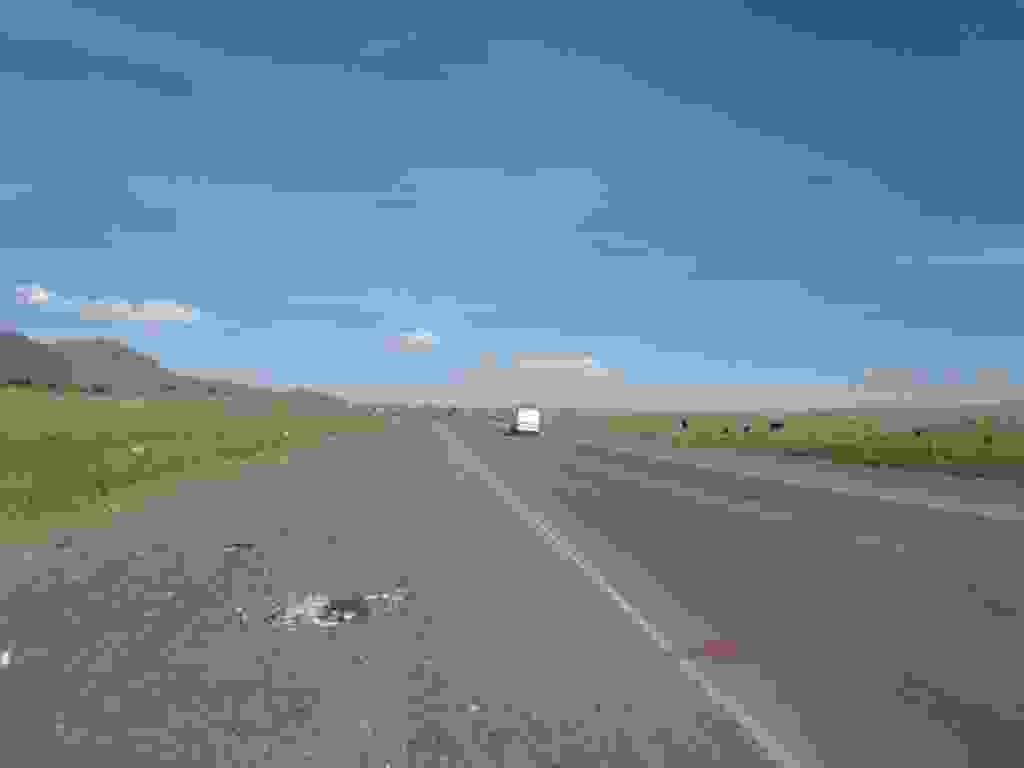
\includegraphics[width=\mywidth]{../wp-content/uploads/2015/05/wpid-wp-1431979840835-1024x768.jpg} \end{center}

 

 Belle vue sur les sommets enneigés de la Cordillera Real. 

 

\begin{center} 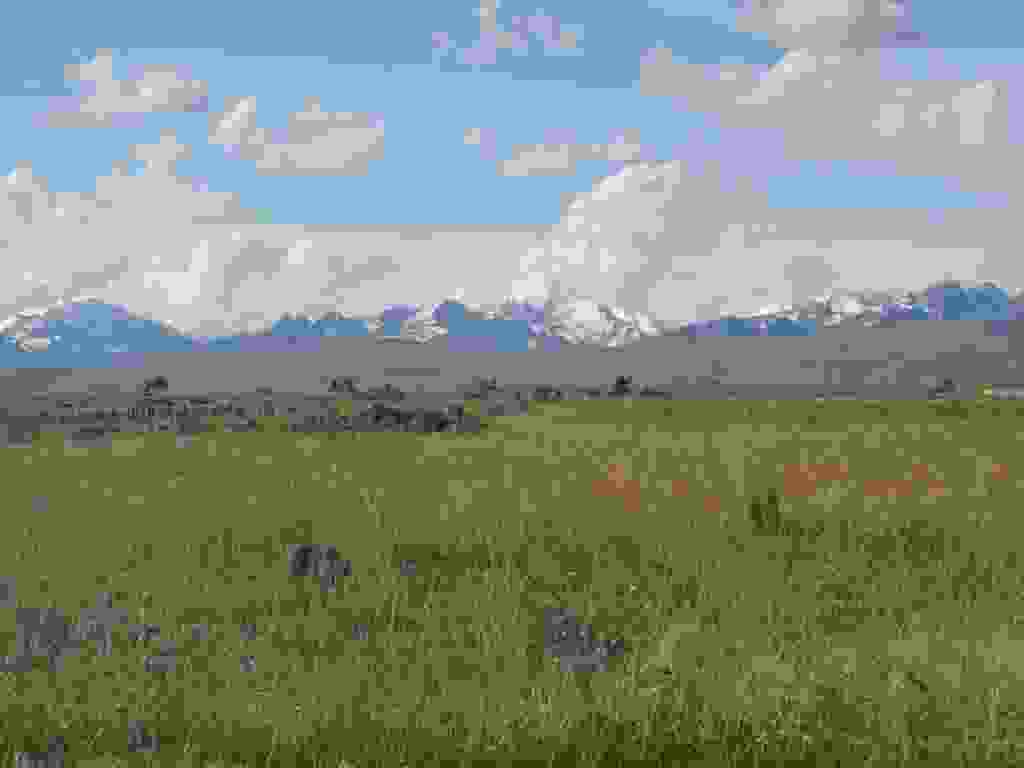
\includegraphics[width=\mywidth]{../wp-content/uploads/2015/05/wpid-wp-1431979897970-1024x768.jpg} \end{center}

 

 

\begin{center} 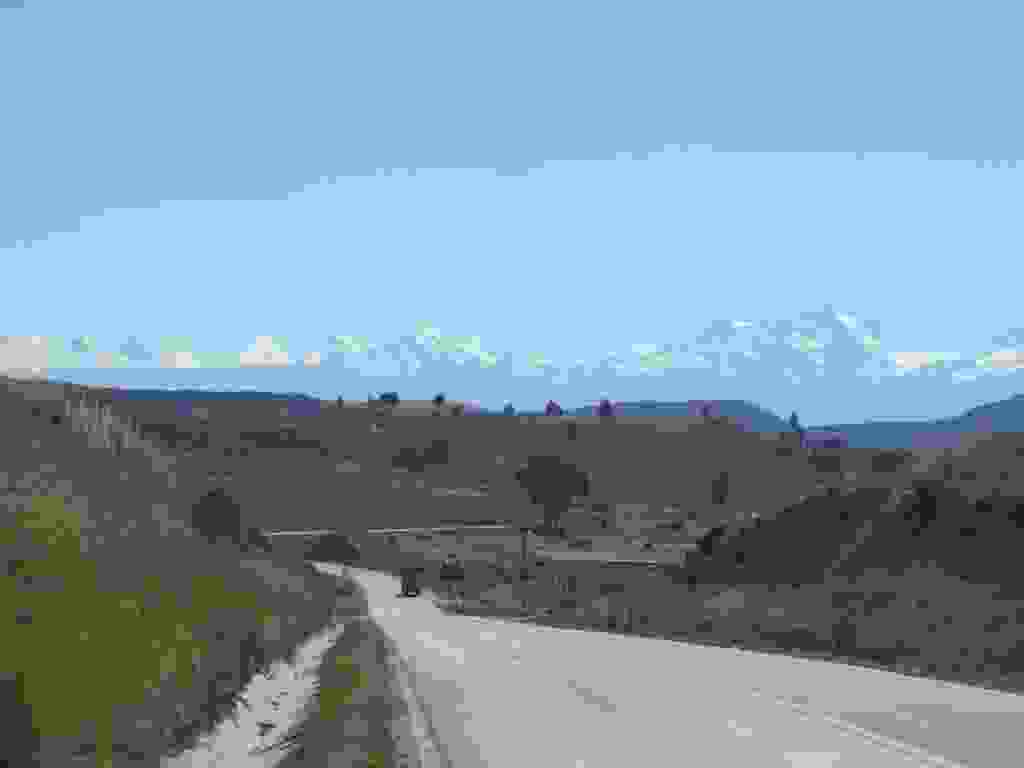
\includegraphics[width=\mywidth]{../wp-content/uploads/2015/05/wpid-wp-1431979933046-1024x768.jpg} \end{center}

 

 Puis la route commence à longer le lac Titicaca. 

 

\begin{center} 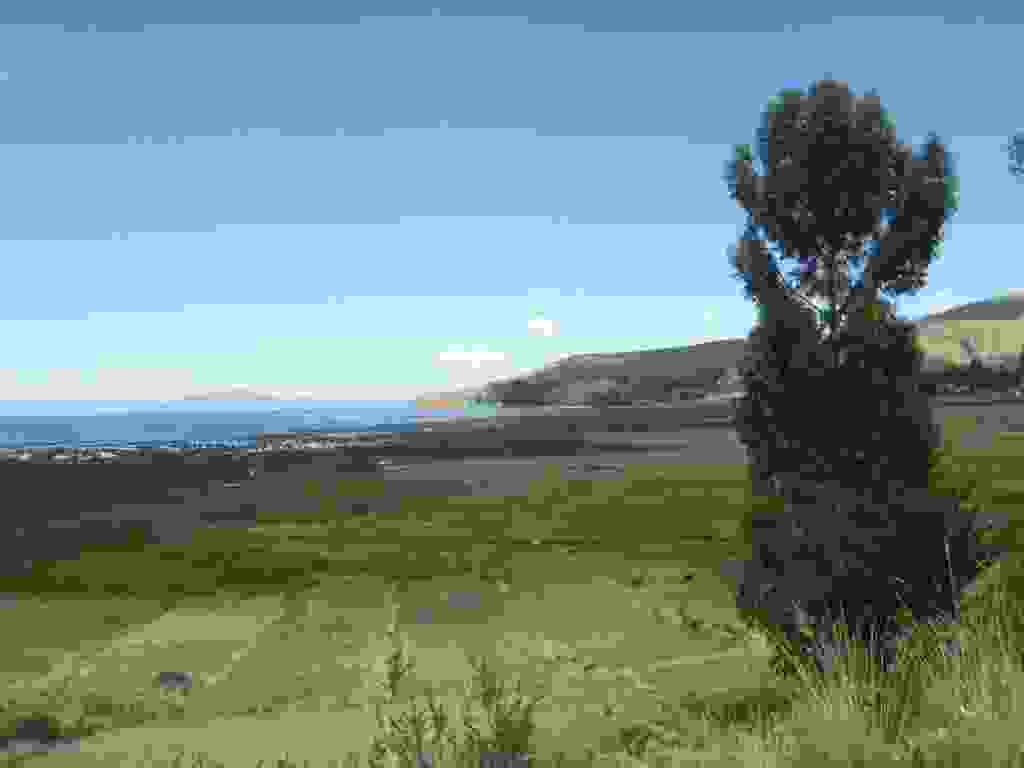
\includegraphics[width=\mywidth]{../wp-content/uploads/2015/05/wpid-wp-1431980026196-1024x768.jpg} \end{center}

 

 

\begin{center} 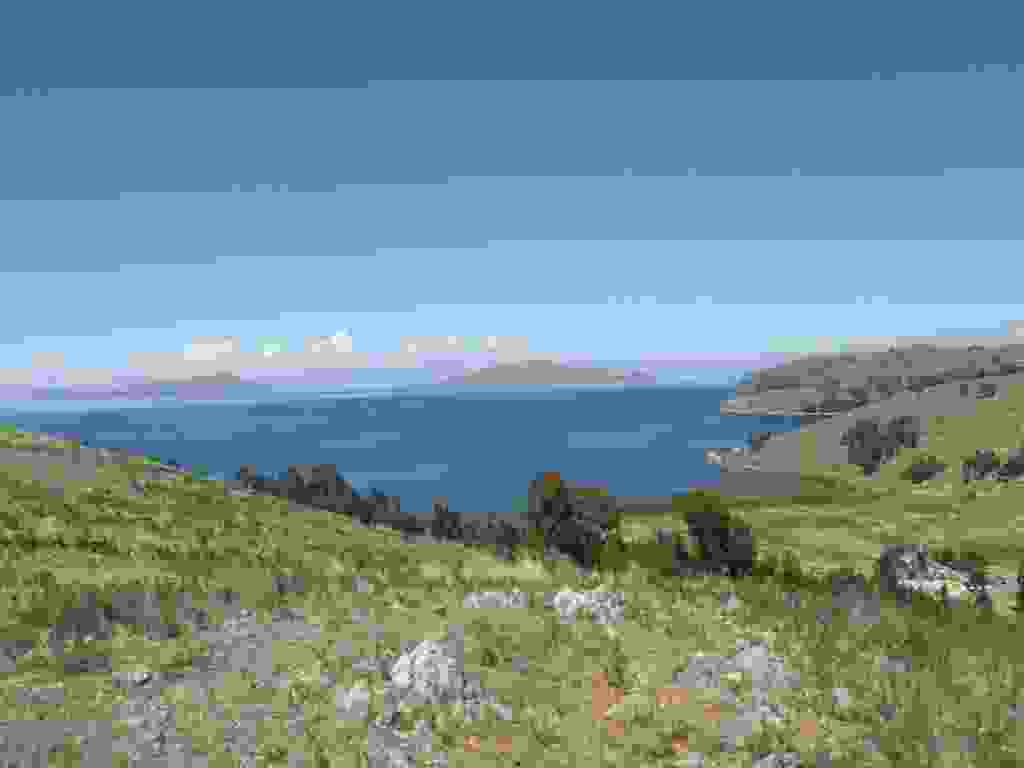
\includegraphics[width=\mywidth]{../wp-content/uploads/2015/05/wpid-wp-1431980086347-1024x768.jpg} \end{center}

 

 

\begin{center} 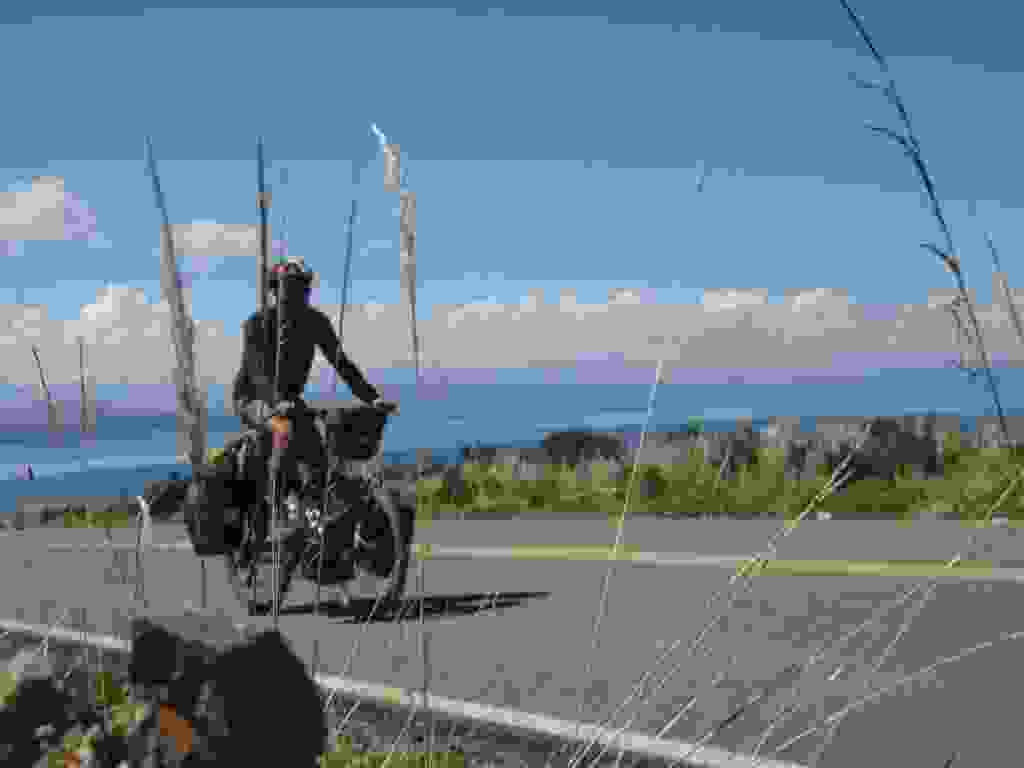
\includegraphics[width=\mywidth]{../wp-content/uploads/2015/05/wpid-wp-1431980142946-1024x768.jpg} \end{center}

 

 

\begin{center} 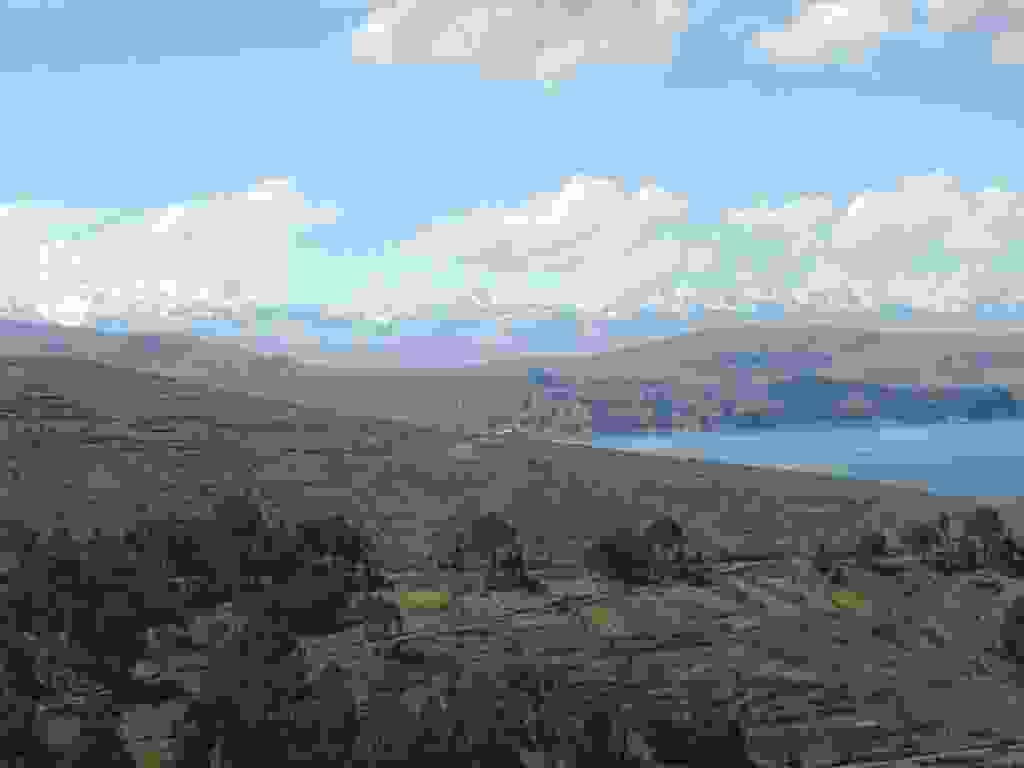
\includegraphics[width=\mywidth]{../wp-content/uploads/2015/05/wpid-wp-1431980233835-1024x768.jpg} \end{center}

 

 Un petit bac permet de traverser le lac entre San Pablo de Tiquina et San Pedro de Tiquina. 

 

\begin{center} 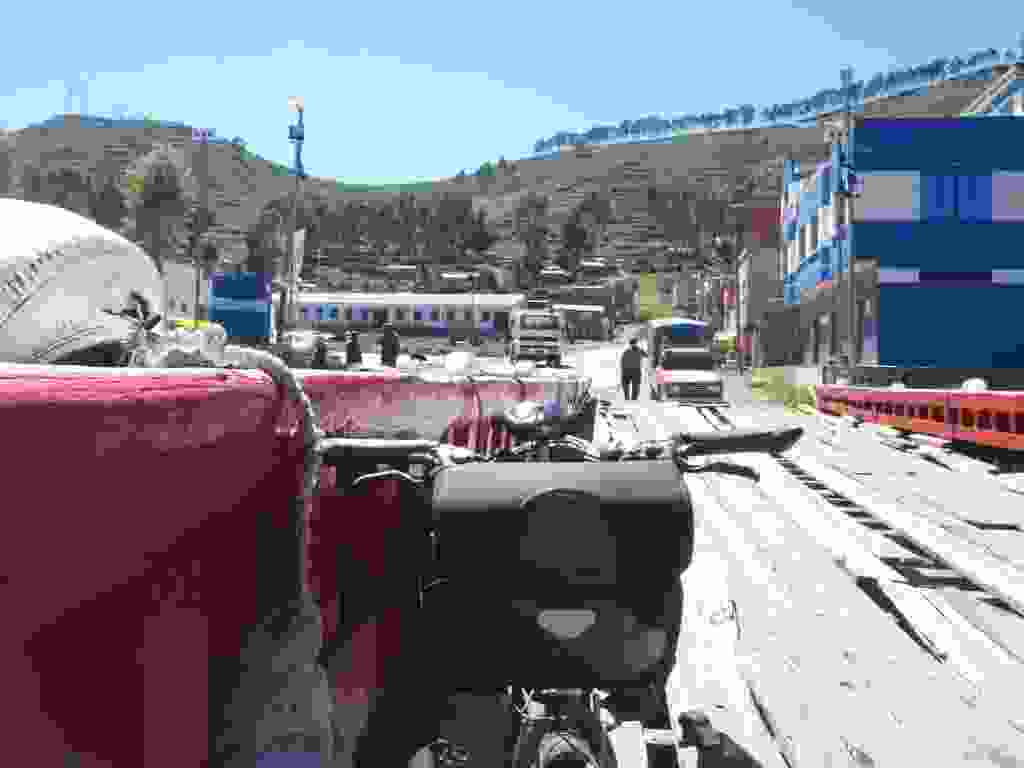
\includegraphics[width=\mywidth]{../wp-content/uploads/2015/05/wpid-wp-1431980249161-1024x768.jpg} \end{center}

 

 Après midi de vélo magnifique avec vues sur le lac parfois des 2 côtés de la route. 

 

\begin{center} 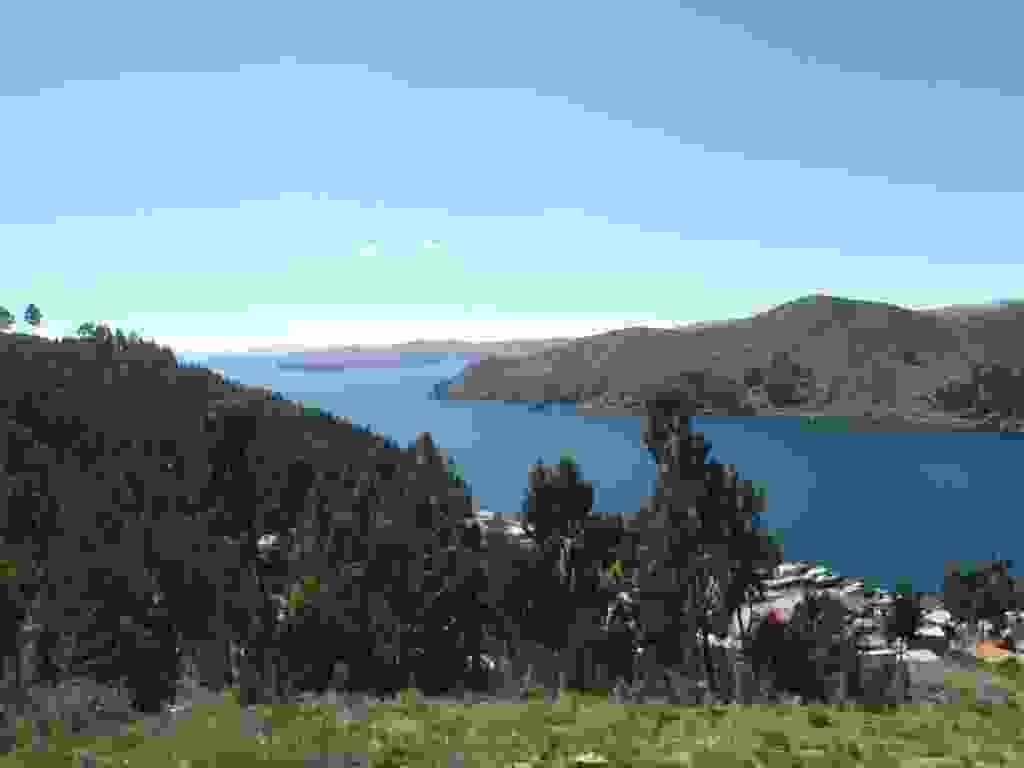
\includegraphics[width=\mywidth]{../wp-content/uploads/2015/05/wpid-wp-1431980351124-1024x768.jpg} \end{center}

 

 

\begin{center} 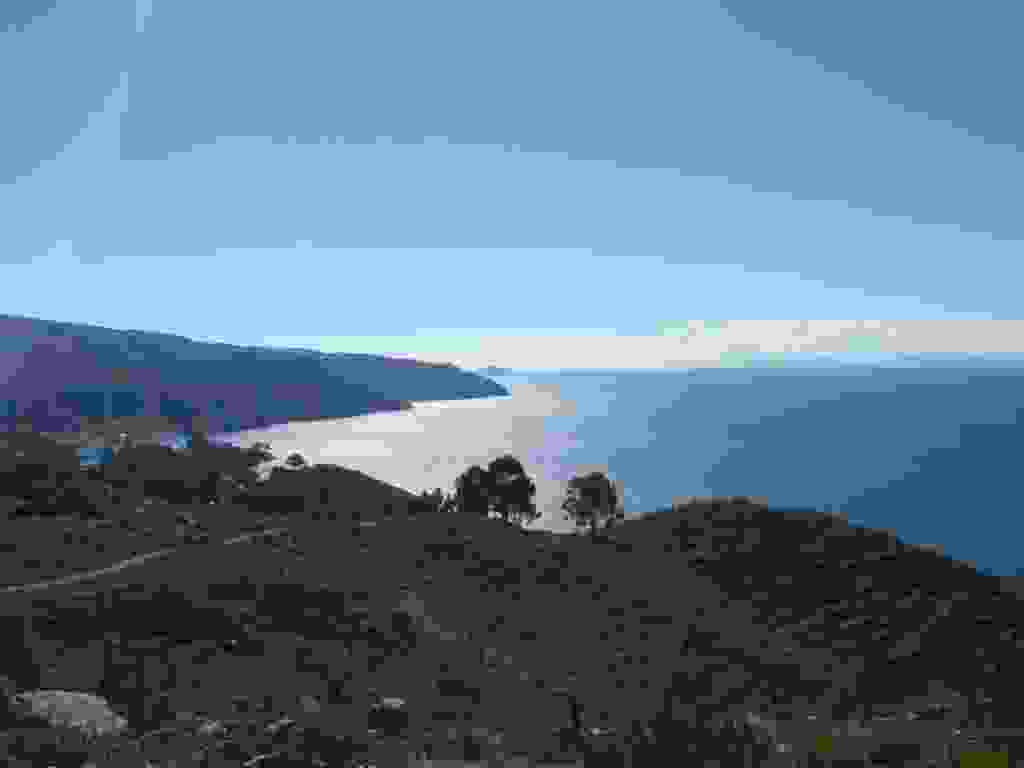
\includegraphics[width=\mywidth]{../wp-content/uploads/2015/05/wpid-wp-1431980399787-1024x768.jpg} \end{center}

 

 

\begin{center} 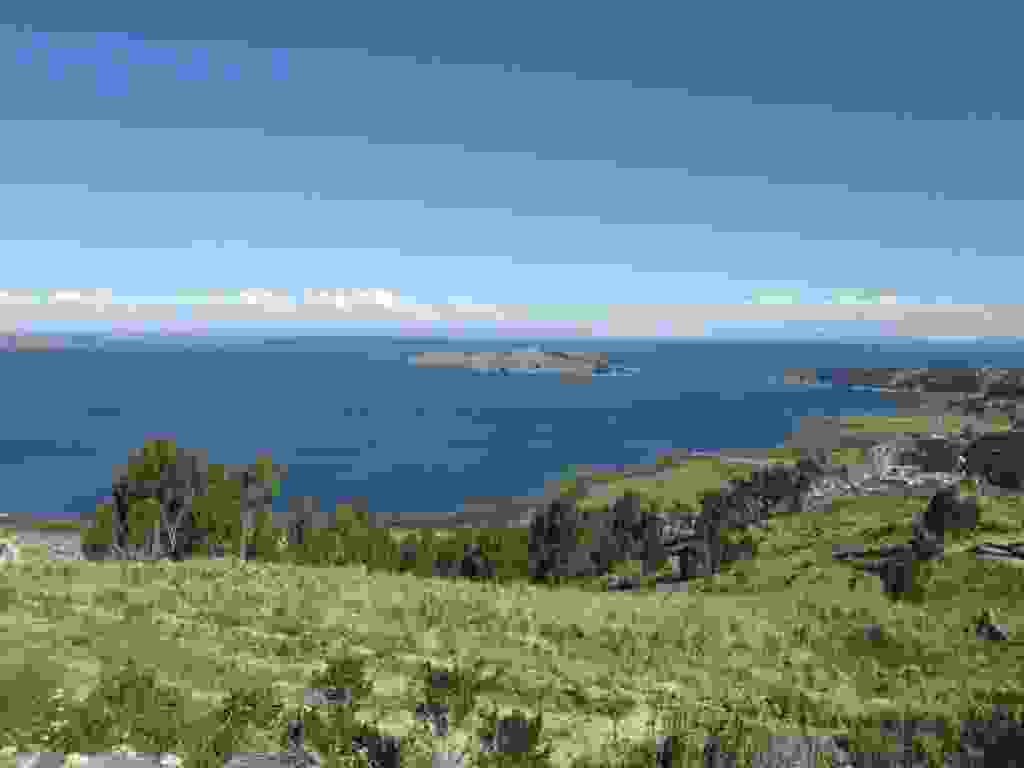
\includegraphics[width=\mywidth]{../wp-content/uploads/2015/05/wpid-wp-1431980460849-1024x768.jpg} \end{center}

 

 La journée se termine par une superbe descente sur Copacabana. 

 

\begin{center} 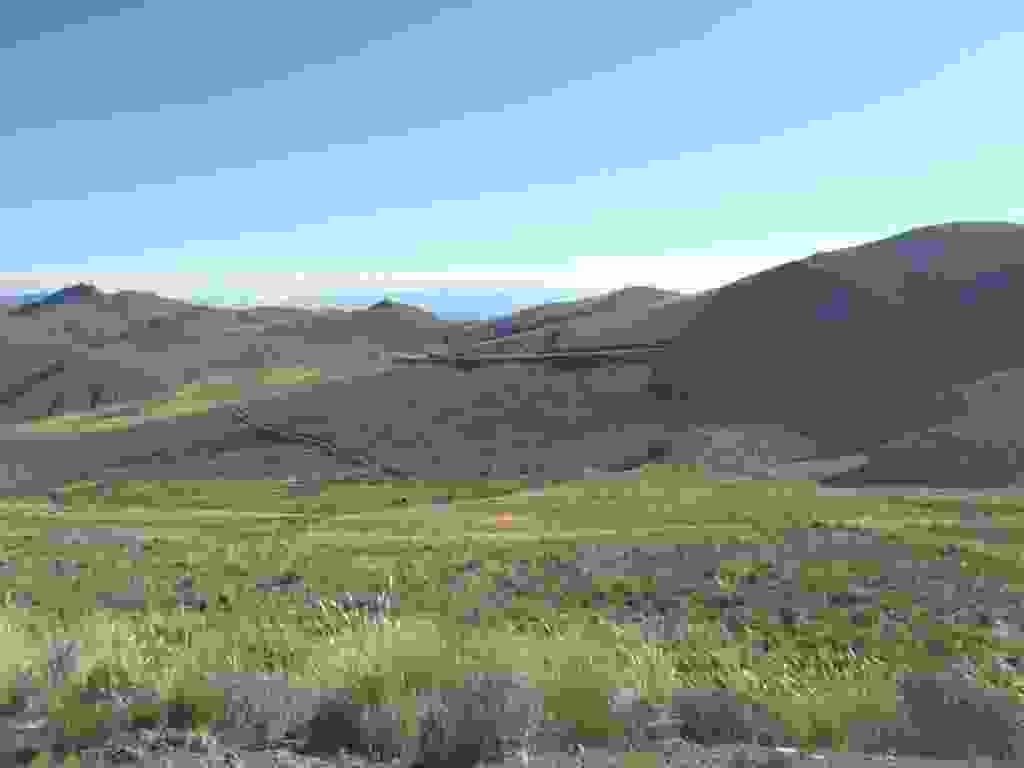
\includegraphics[width=\mywidth]{../wp-content/uploads/2015/05/wpid-wp-1431980488414-1024x768.jpg} \end{center}

 

 

\begin{center} 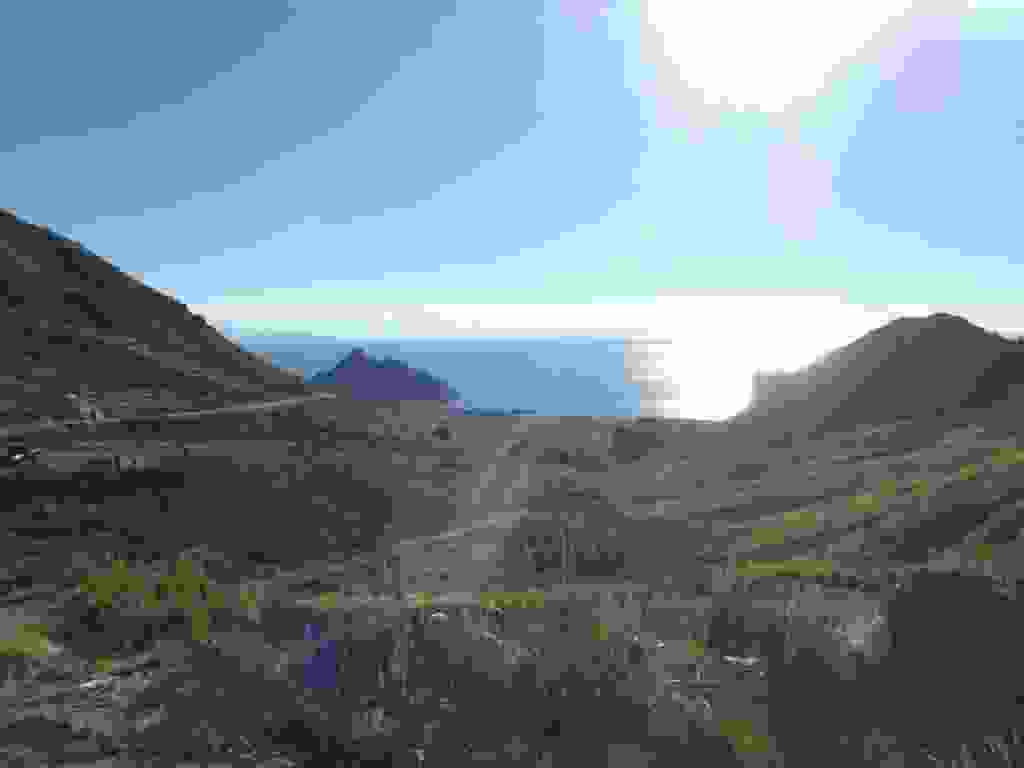
\includegraphics[width=\mywidth]{../wp-content/uploads/2015/05/wpid-wp-1431980538500-1024x768.jpg} \end{center}

 

 

\begin{center} 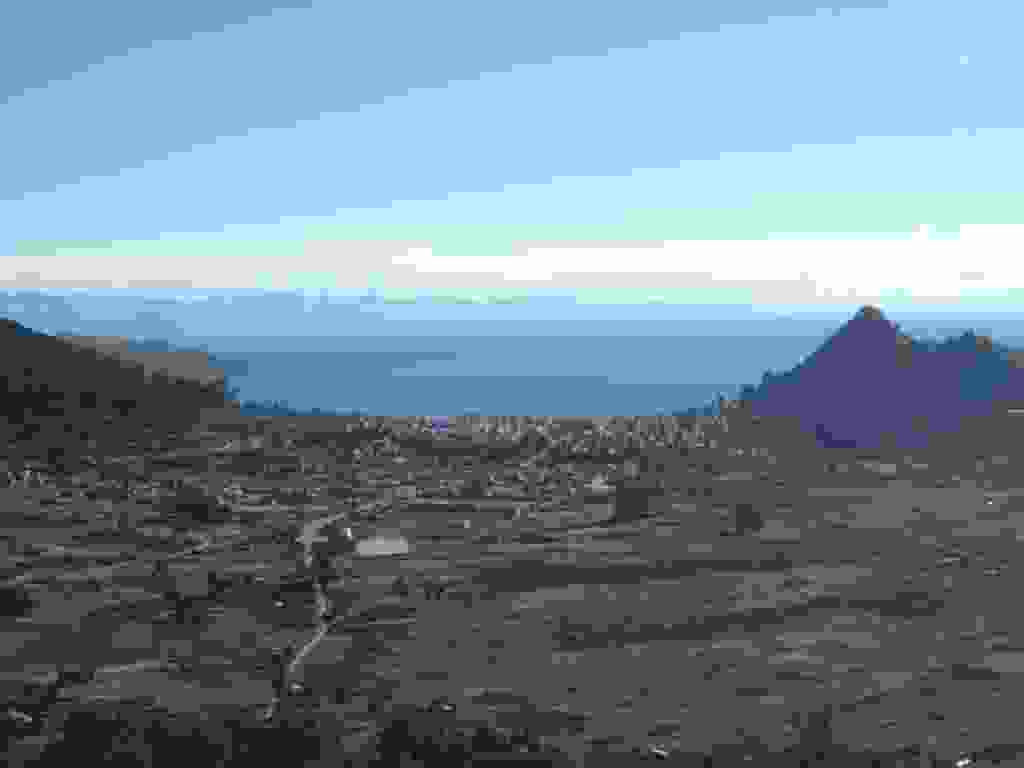
\includegraphics[width=\mywidth]{../wp-content/uploads/2015/05/wpid-wp-1431980616756-1024x768.jpg} \end{center}

 

 C'est une ville de pèlerinage pour les Boliviens qui viennent bénir leurs objets au sommet du calvaire. 

 

\begin{center} 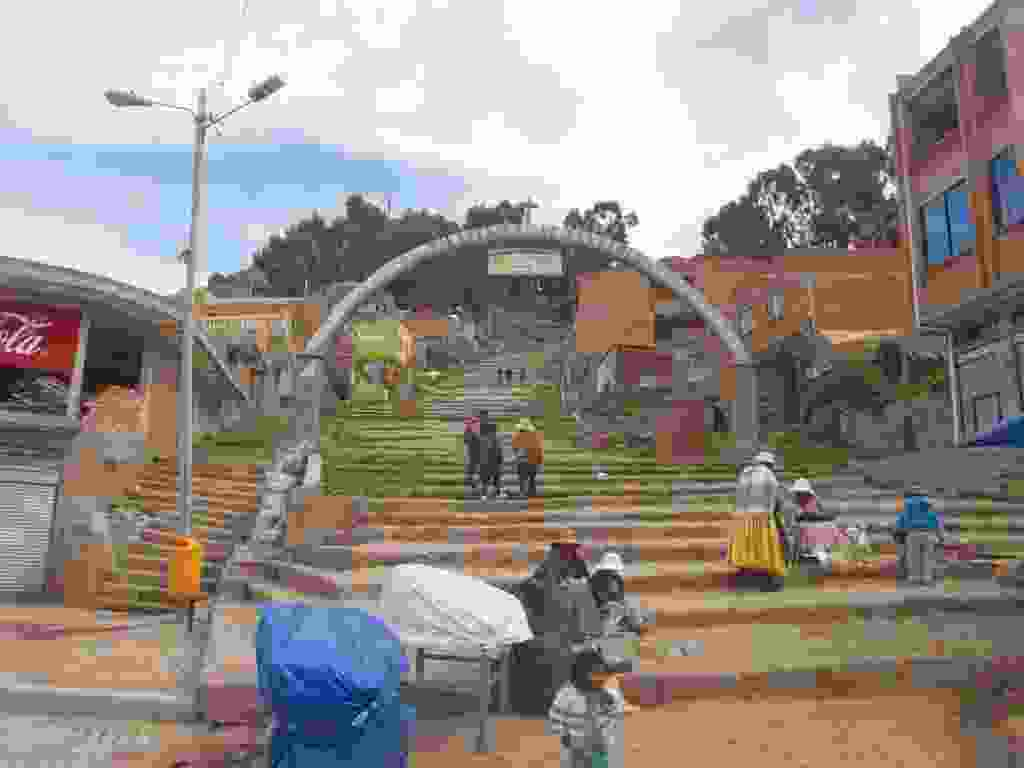
\includegraphics[width=\mywidth]{../wp-content/uploads/2015/05/wpid-wp-1431980662233-1024x768.jpg} \end{center}

 

 

\begin{center} 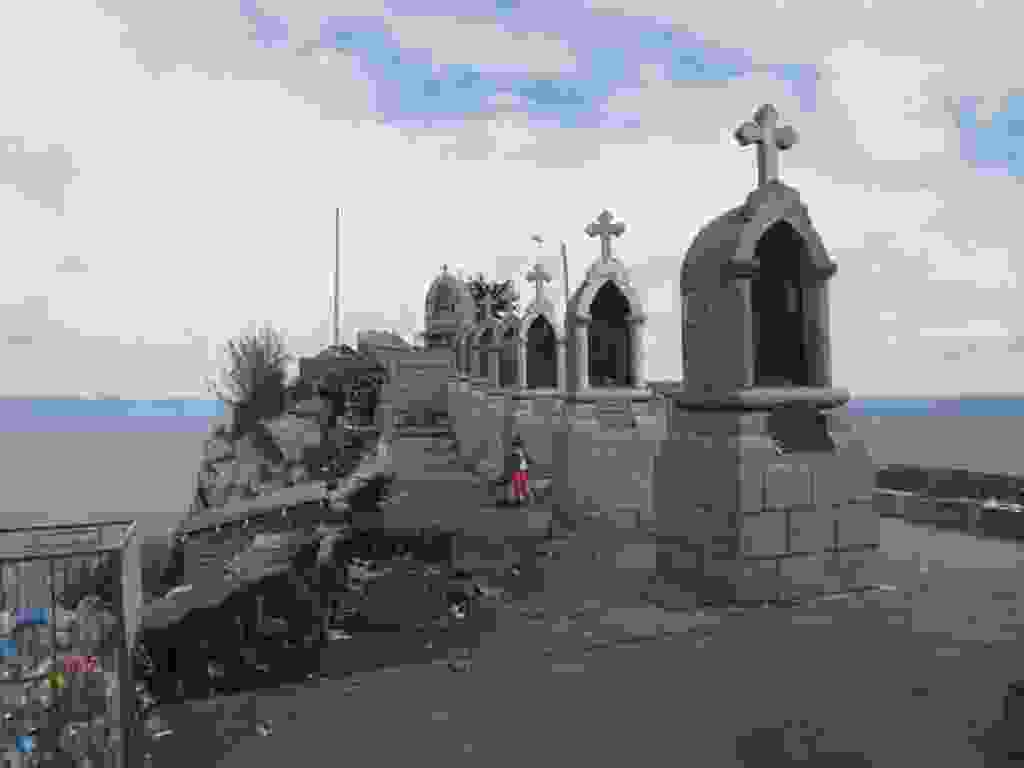
\includegraphics[width=\mywidth]{../wp-content/uploads/2015/05/wpid-wp-1431980676492-1024x768.jpg} \end{center}

 

 

\begin{center} 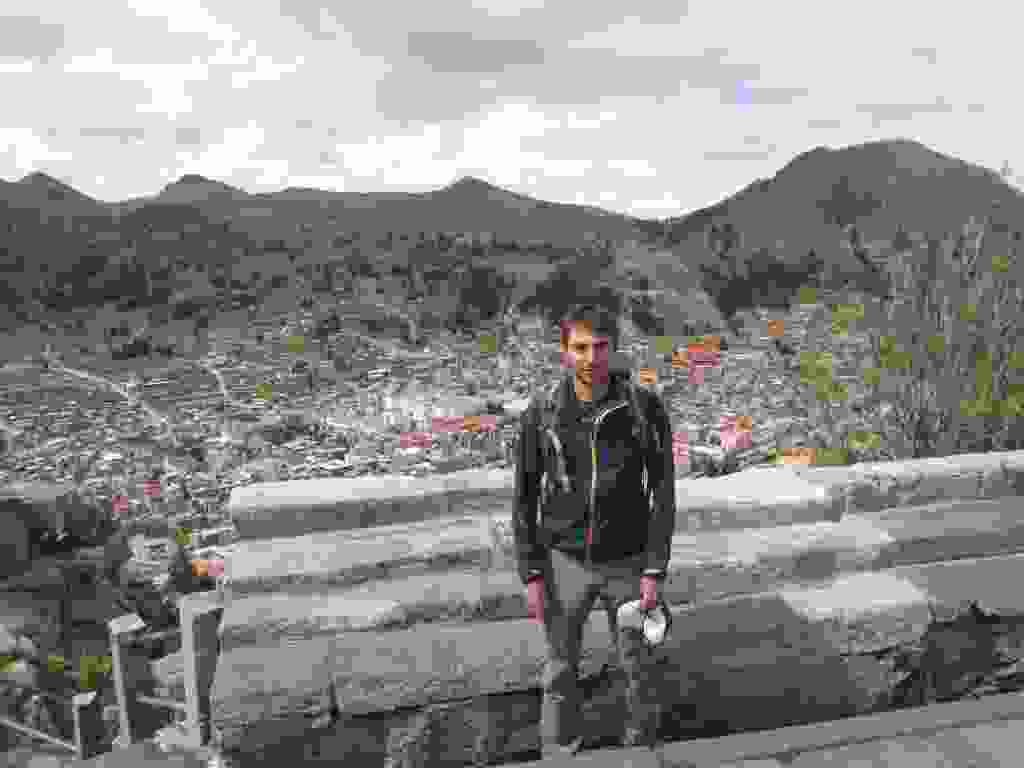
\includegraphics[width=\mywidth]{../wp-content/uploads/2015/05/wpid-wp-1431980730580-1024x768.jpg} \end{center}

 

 

\begin{center} 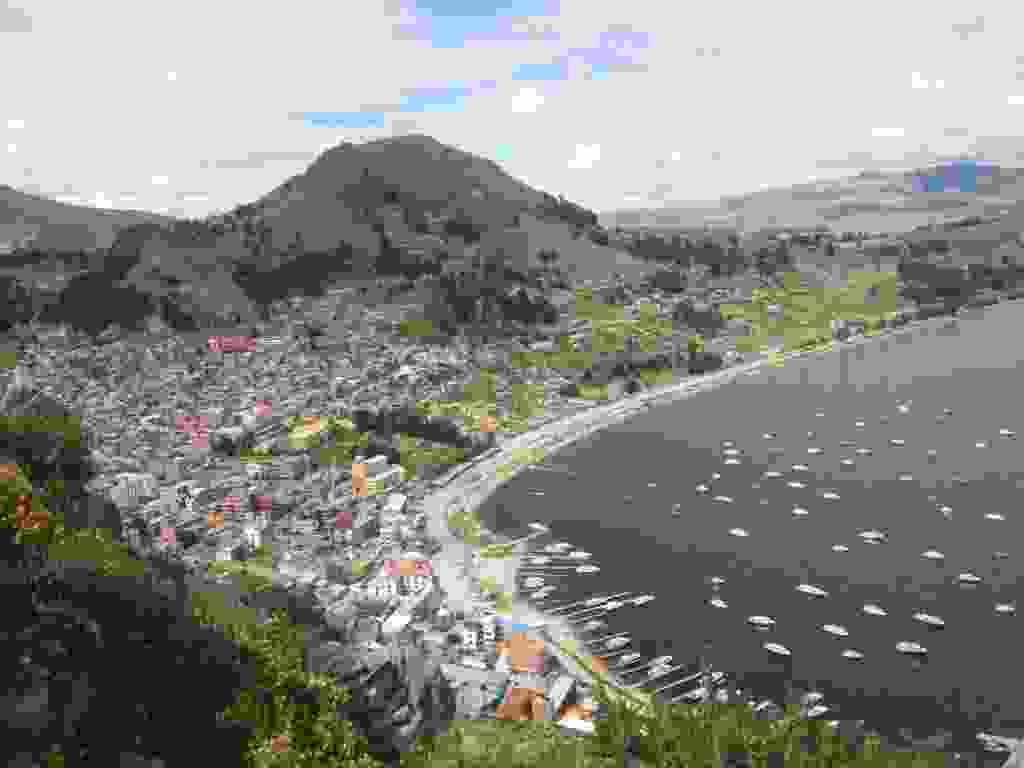
\includegraphics[width=\mywidth]{../wp-content/uploads/2015/05/wpid-wp-1431980752649-1024x768.jpg} \end{center}

 

 C'est une ville très touristique, remplie d'hôtels, de restaurants et de boutiques de souvenirs. 

 

\begin{center} 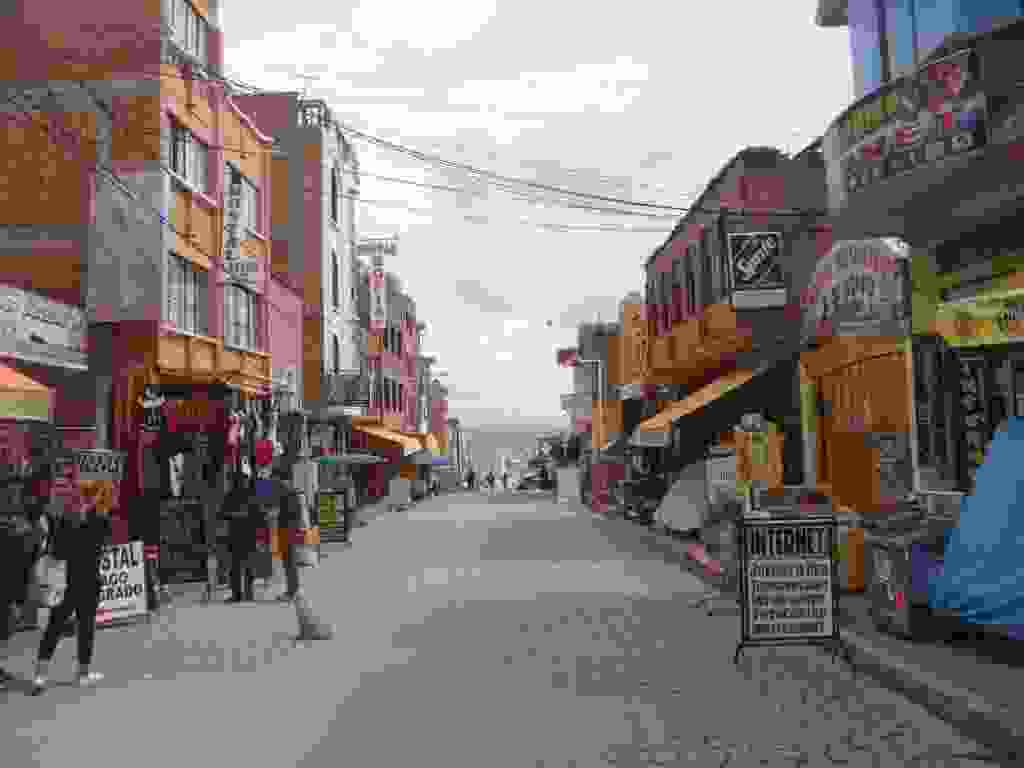
\includegraphics[width=\mywidth]{../wp-content/uploads/2015/05/wpid-wp-1431980819257-1024x768.jpg} \end{center}

 

 La truite grillée du lac est très bonne et pour à peine plus de 3 euros. 

 

\begin{center} 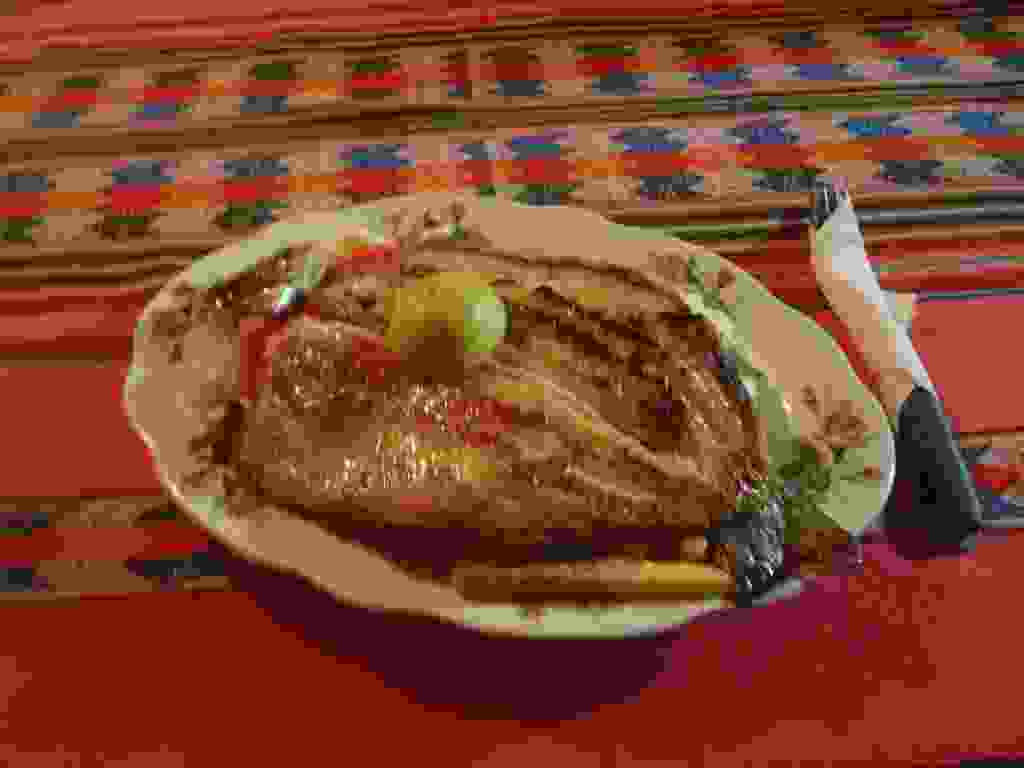
\includegraphics[width=\mywidth]{../wp-content/uploads/2015/05/wpid-wp-1431980877471-1024x768.jpg} \end{center}

 

 En face de Copacabana se trouve l'Isla del Sol à 2h de bateau. 

 

\begin{center} 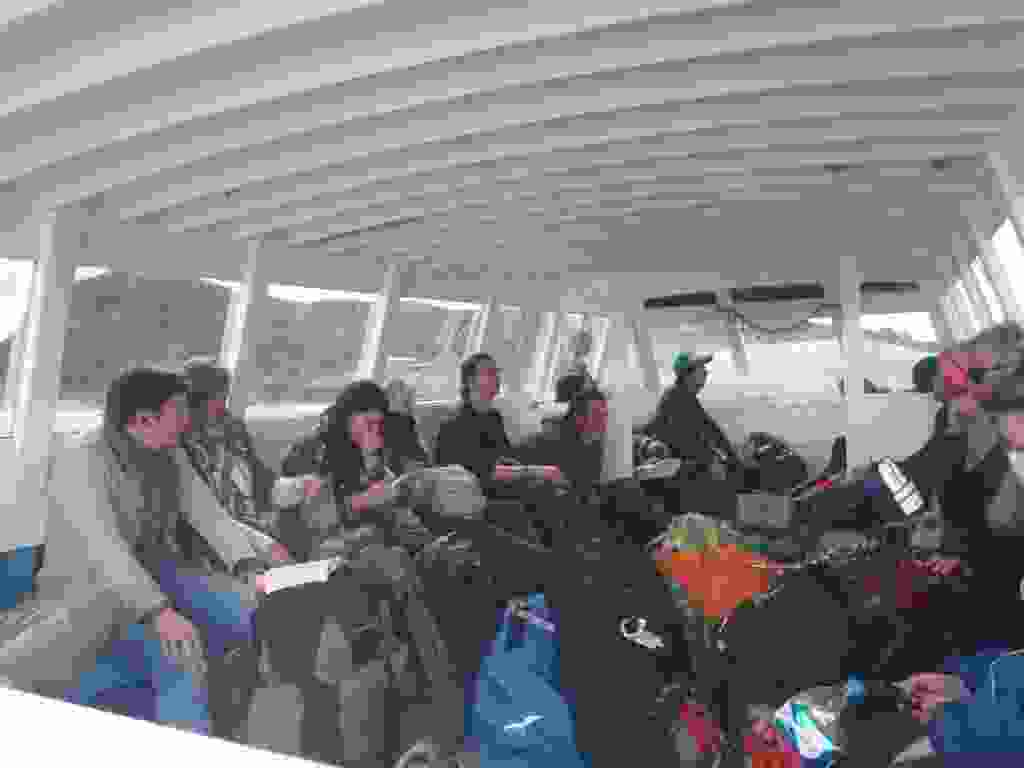
\includegraphics[width=\mywidth]{../wp-content/uploads/2015/05/wpid-wp-1432046789710-1024x768.jpg} \end{center}

 

 C'est une petite île très calme, pas de voiture. 

 

\begin{center} 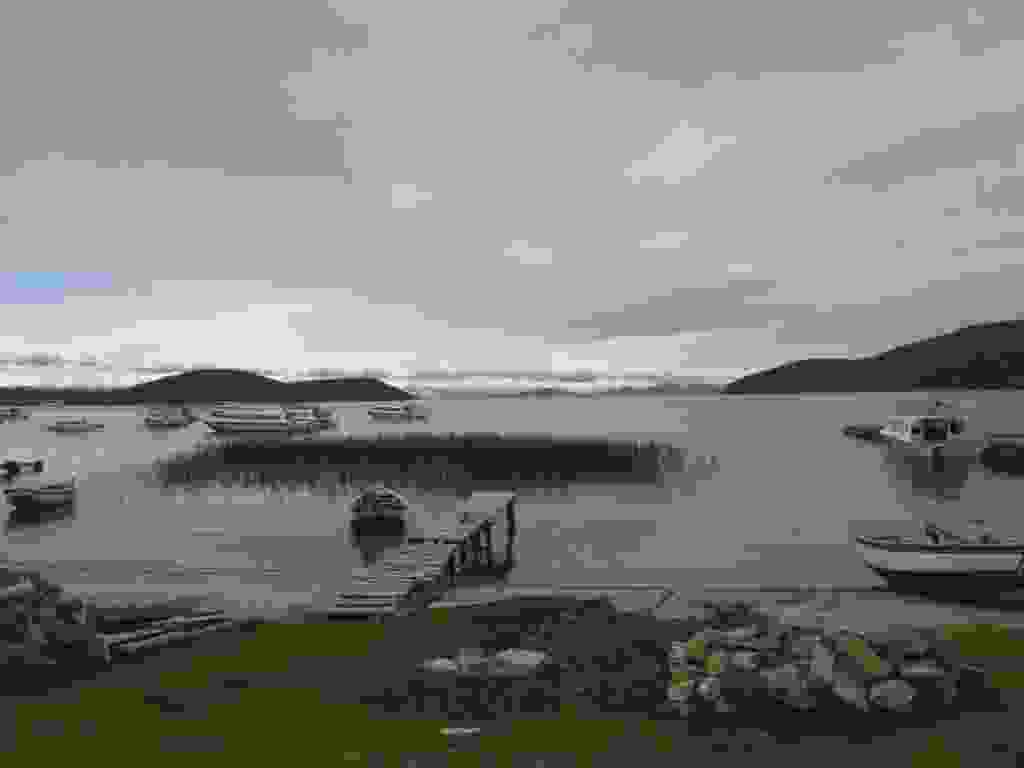
\includegraphics[width=\mywidth]{../wp-content/uploads/2015/05/P5073888-1024x768.jpg} \end{center}

 

 

\begin{center} 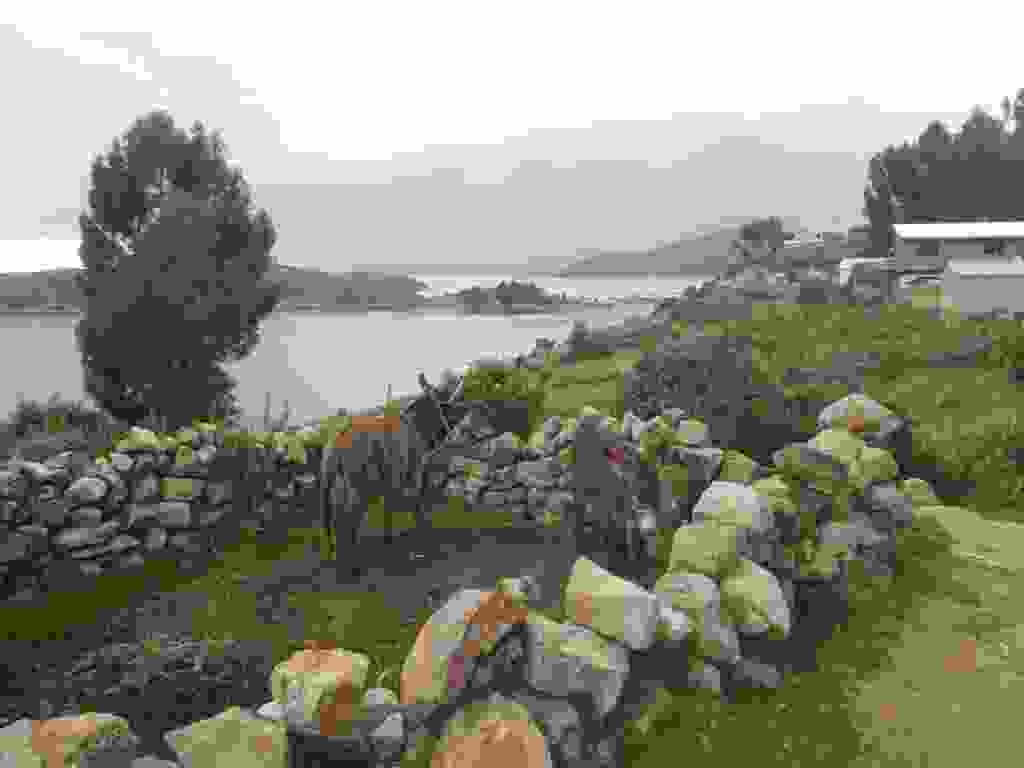
\includegraphics[width=\mywidth]{../wp-content/uploads/2015/05/wpid-wp-1432046835096-1024x768.jpg} \end{center}

 

 

\begin{center} 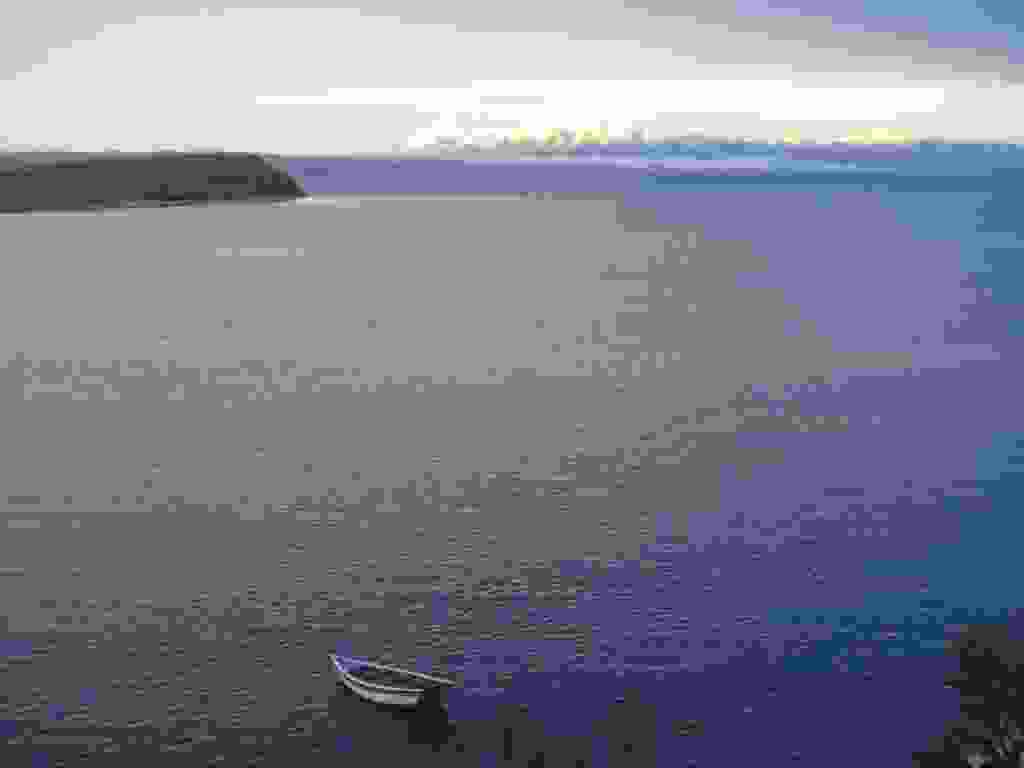
\includegraphics[width=\mywidth]{../wp-content/uploads/2015/05/wpid-wp-1432046850969-1024x768.jpg} \end{center}

 

 

\begin{center} 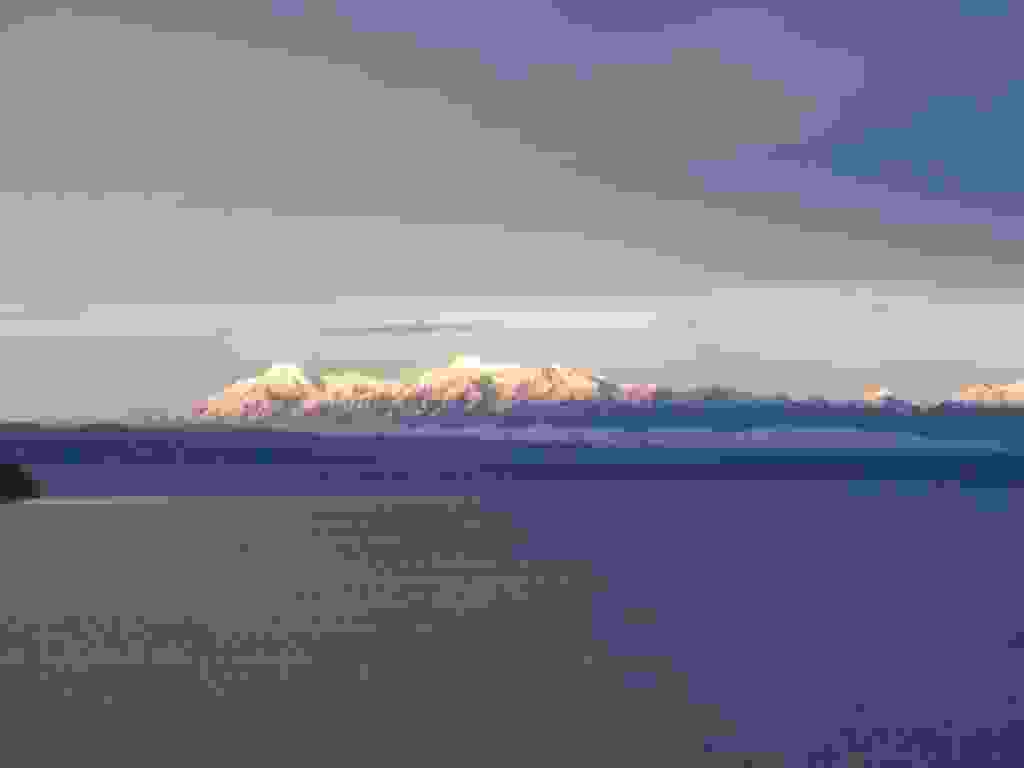
\includegraphics[width=\mywidth]{../wp-content/uploads/2015/05/wpid-wp-1432046865328-1024x768.jpg} \end{center}

 

 Les habitants semblent toujours porter quelque chose. 

 

\begin{center} 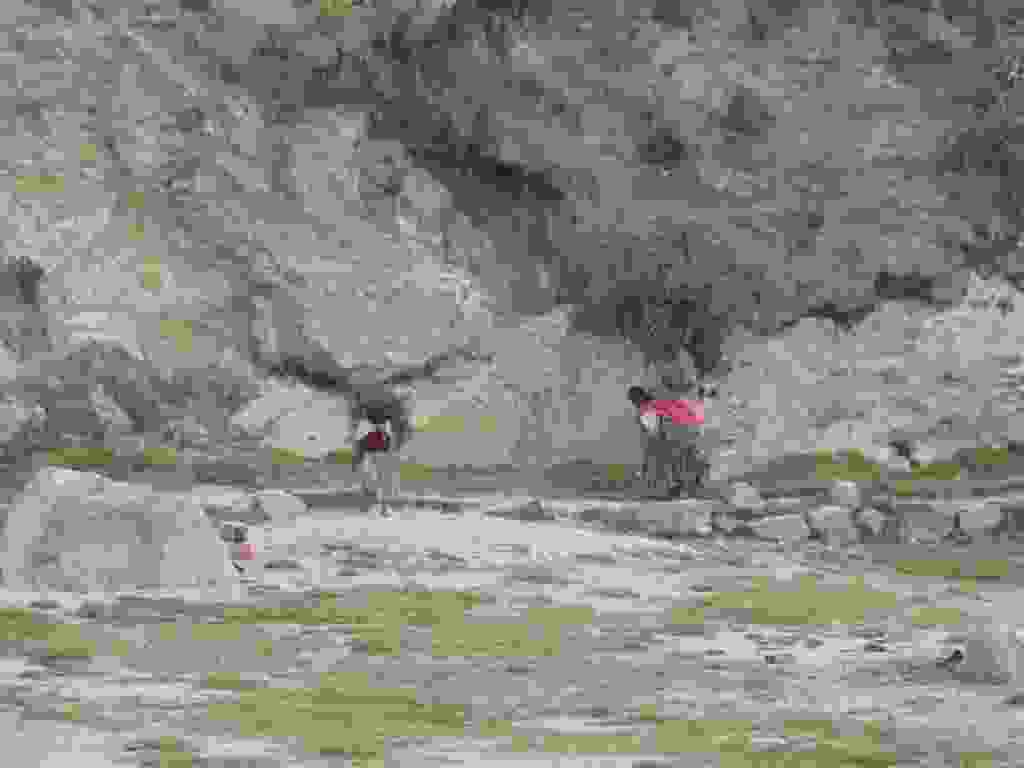
\includegraphics[width=\mywidth]{../wp-content/uploads/2015/05/wpid-wp-1432046915574-1024x768.jpg} \end{center}

 

 Un site inca au nord de l'île. 

 

\begin{center} 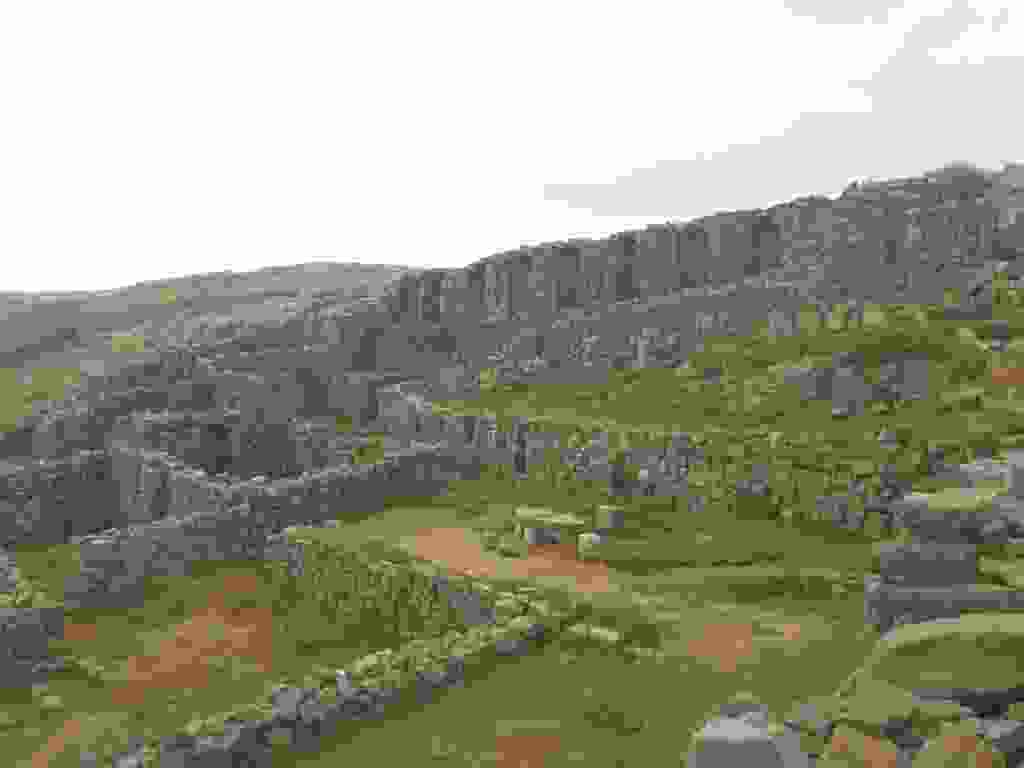
\includegraphics[width=\mywidth]{../wp-content/uploads/2015/05/wpid-wp-1432046930575-1024x768.jpg} \end{center}

 

 Belle balade du nord au sud de l'île, même si le soleil n'était pas trop présent. 

 

\begin{center} 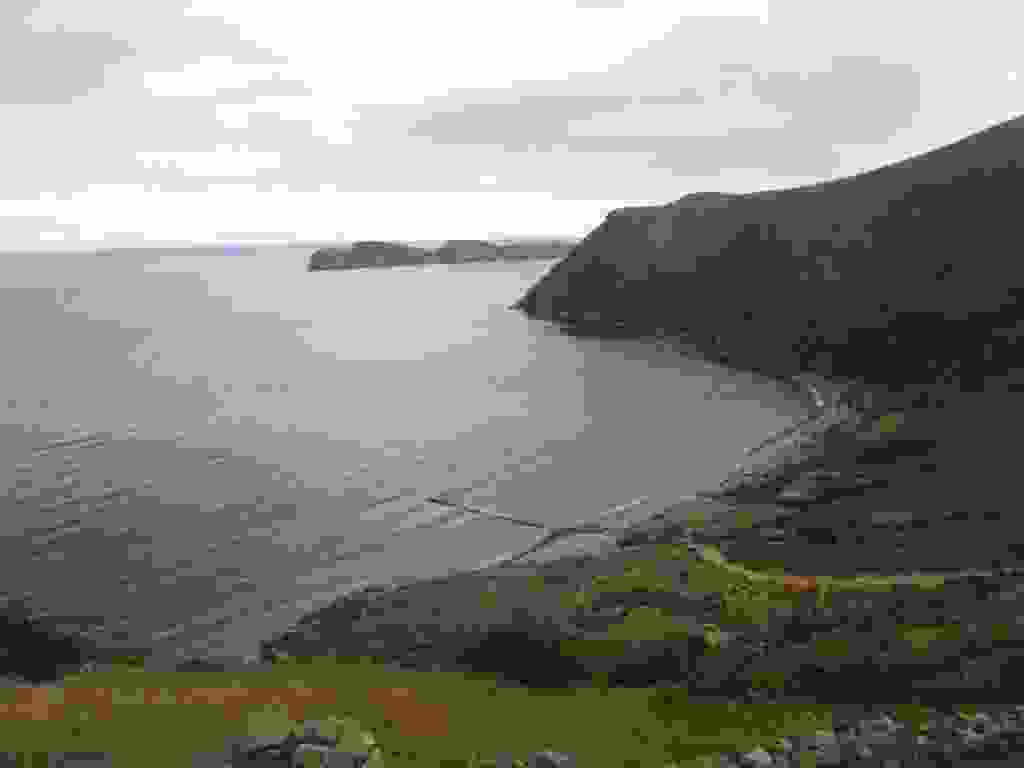
\includegraphics[width=\mywidth]{../wp-content/uploads/2015/05/P5083918-1024x768.jpg} \end{center}

 

 

\begin{center} 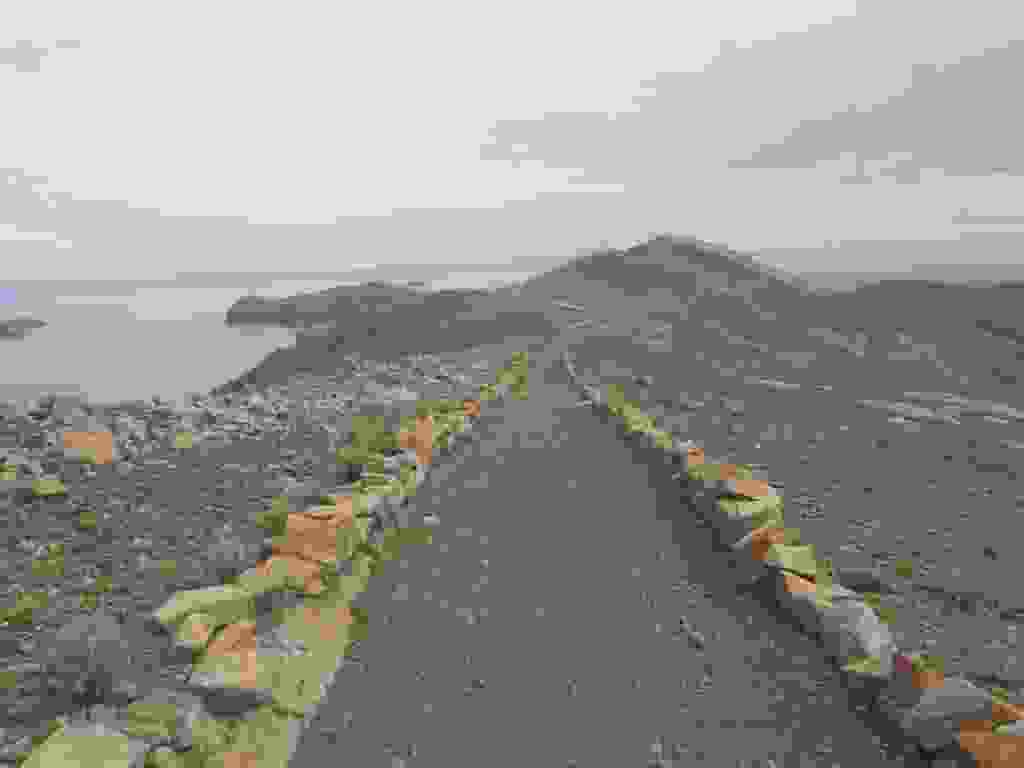
\includegraphics[width=\mywidth]{../wp-content/uploads/2015/05/P5083927-1024x768.jpg} \end{center}

 

 

\begin{center} 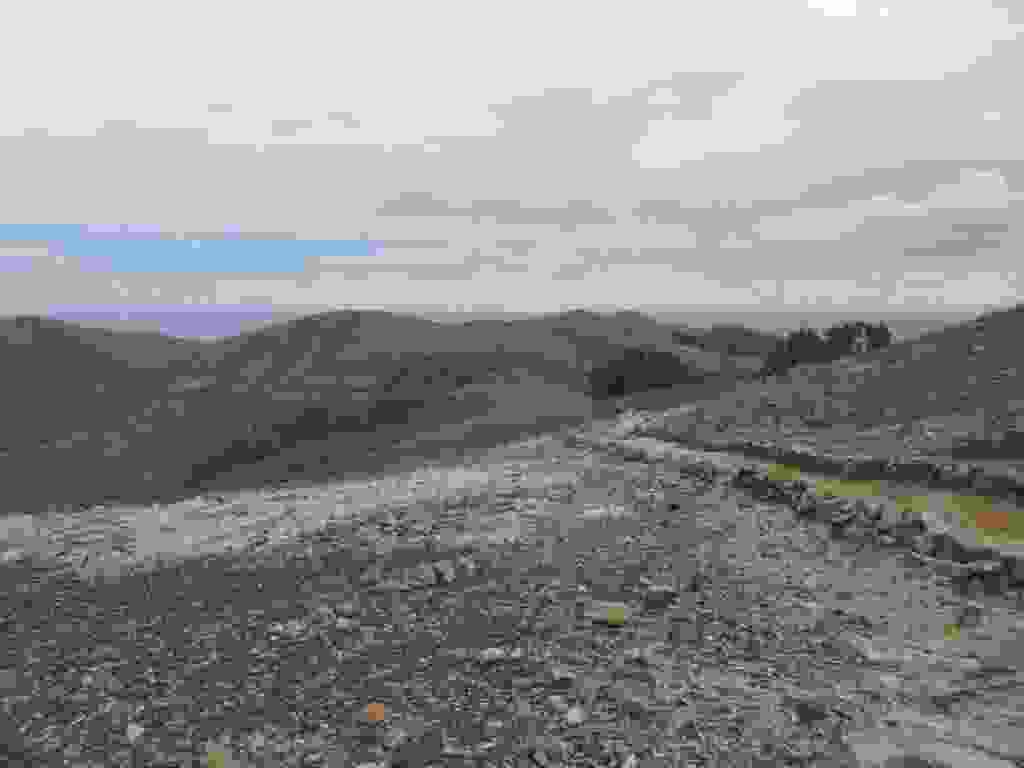
\includegraphics[width=\mywidth]{../wp-content/uploads/2015/05/P5083931-1024x768.jpg} \end{center}

 

 Le réconfort après la marche : une très bonne pizza au quinoa avec vue sur le lac. 

 

\begin{center} 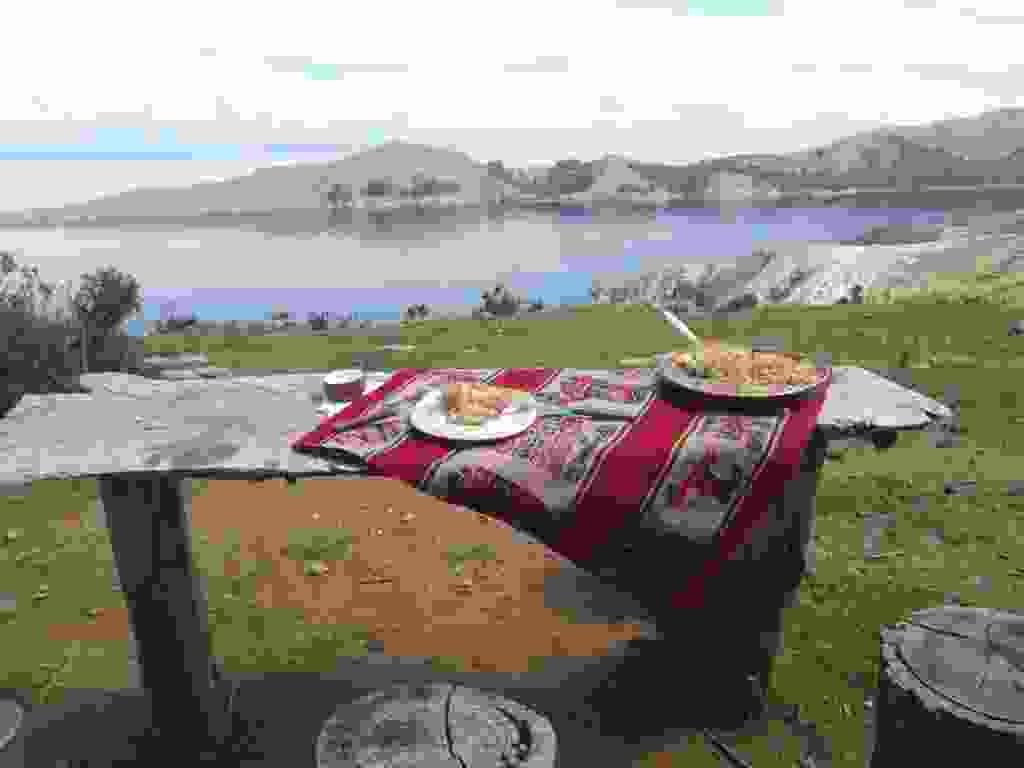
\includegraphics[width=\mywidth]{../wp-content/uploads/2015/05/P5083938-1024x768.jpg} \end{center}

 

 Je continue vers la partie Péruvienne du lac, la frontière est à une dizaine de km de Copacabana. 

 

\begin{center} 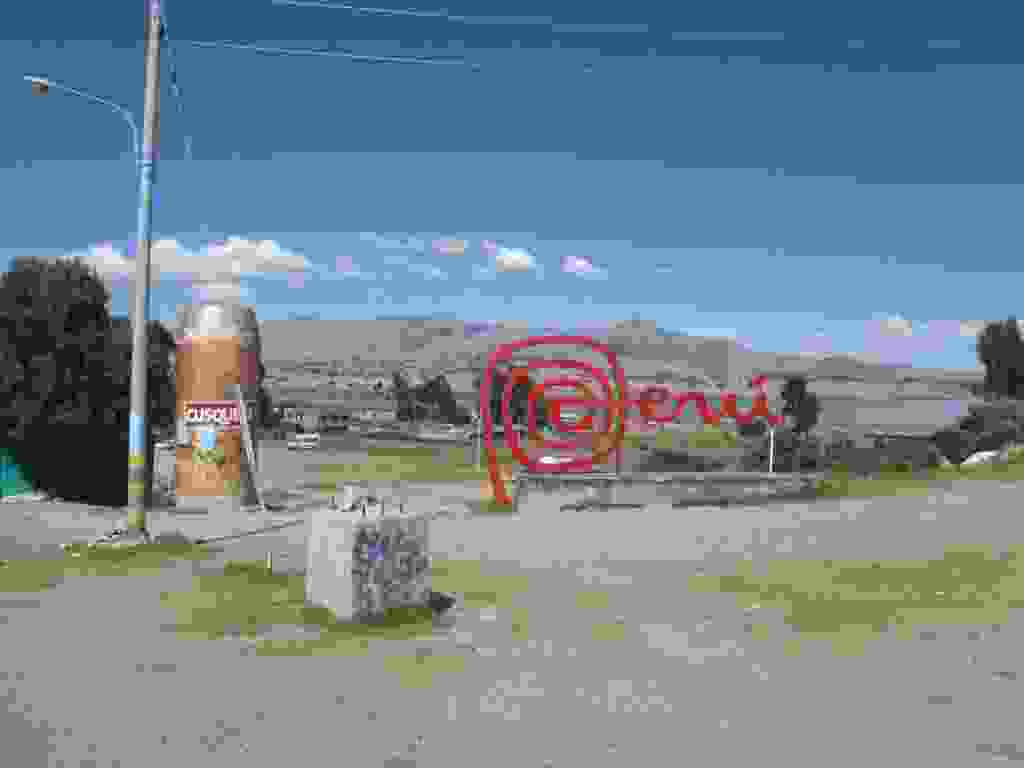
\includegraphics[width=\mywidth]{../wp-content/uploads/2015/05/P5093949-1024x768.jpg} \end{center}

 

 À première vue le Pérou ressemble beaucoup à la Bolivie mais on remarque quand même les triporteurs, omniprésents. 

 

\begin{center} 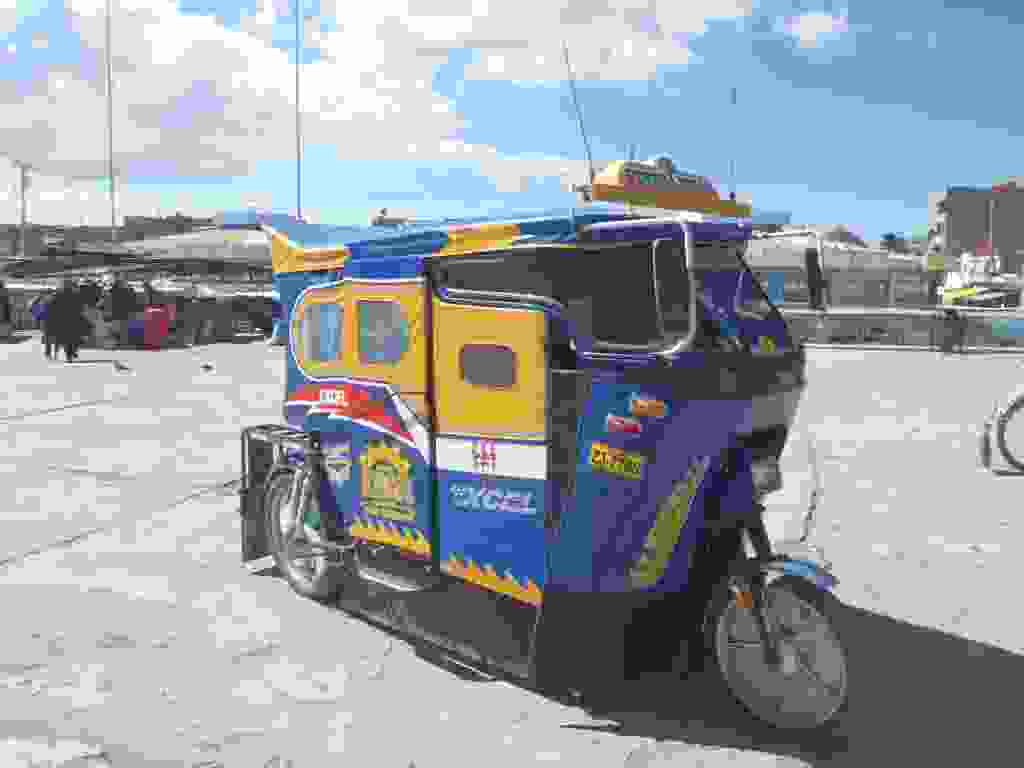
\includegraphics[width=\mywidth]{../wp-content/uploads/2015/05/P5093950-1024x768.jpg} \end{center}

 

 La route continue à longer le lac. 

 

\begin{center} 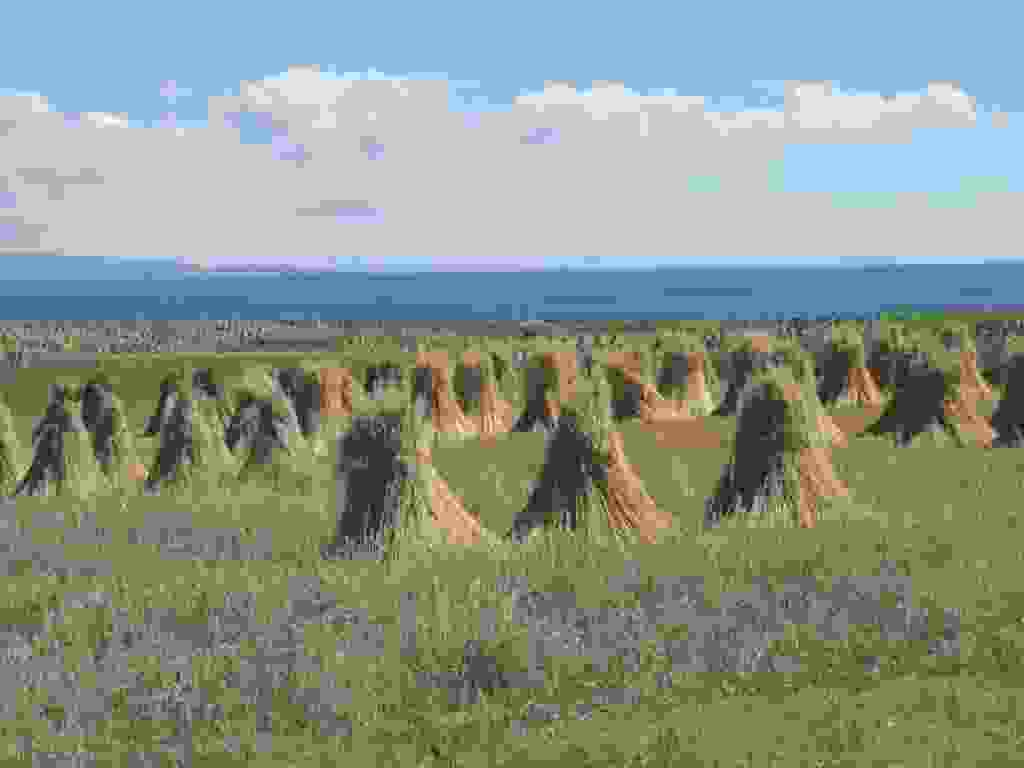
\includegraphics[width=\mywidth]{../wp-content/uploads/2015/05/P5093953-1024x768.jpg} \end{center}

 

 

\begin{center} 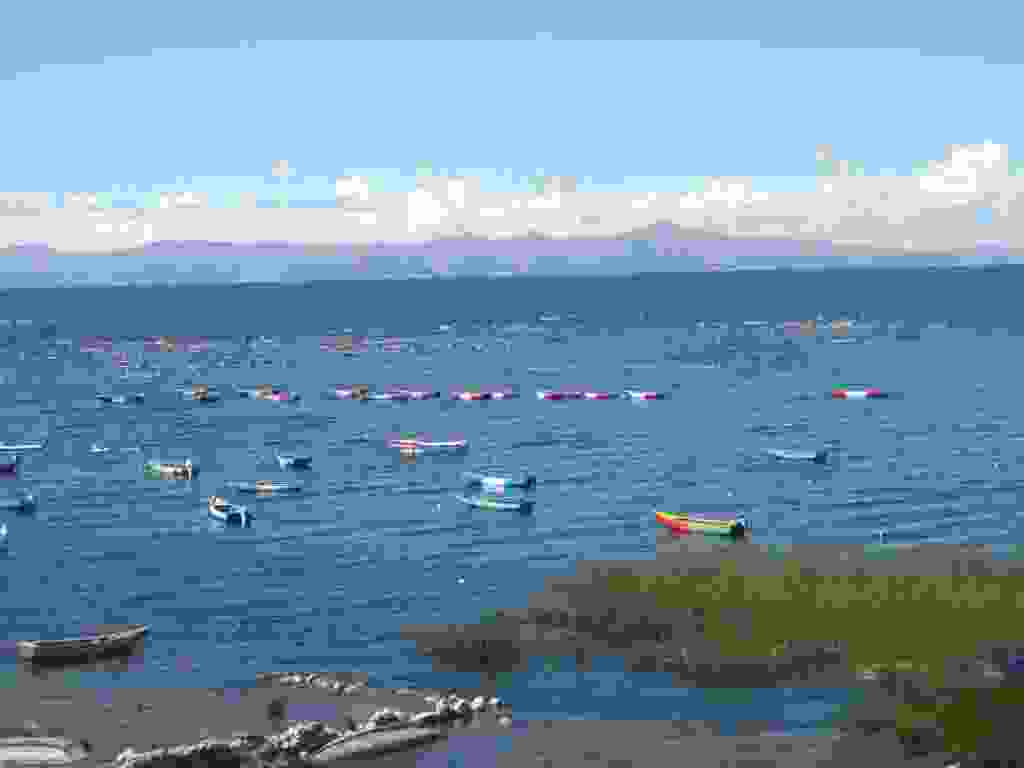
\includegraphics[width=\mywidth]{../wp-content/uploads/2015/05/P5093955-1024x768.jpg} \end{center}

 

 Je m'arrête pour visiter le village de Chucuito. 

 

\begin{center} 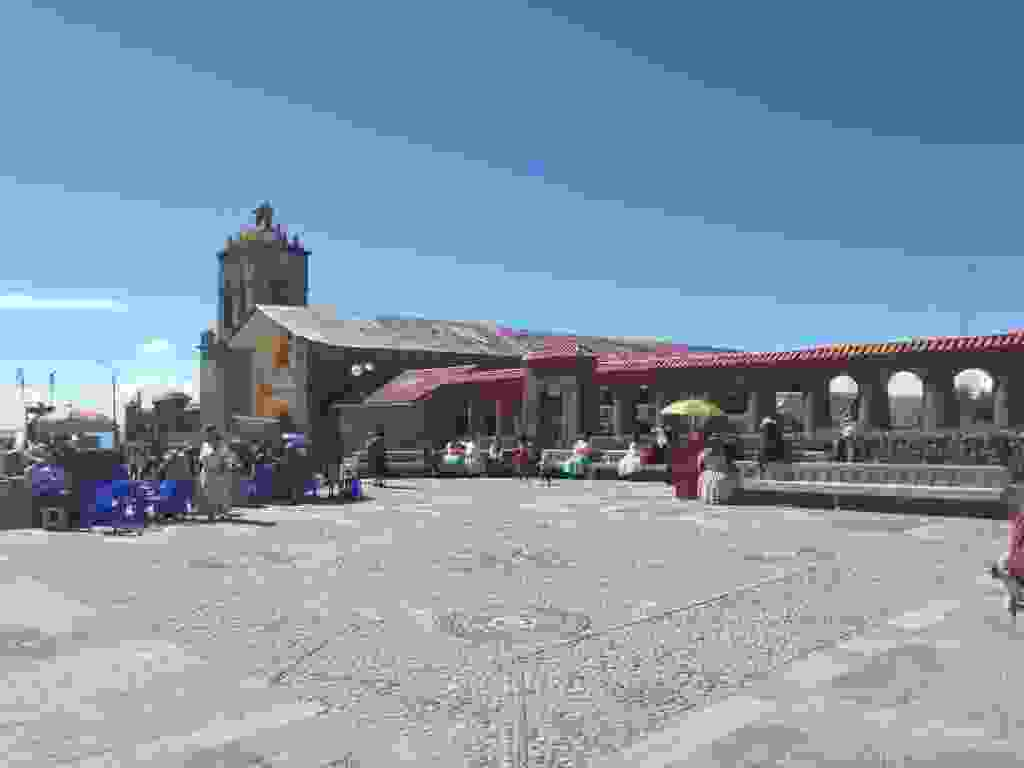
\includegraphics[width=\mywidth]{../wp-content/uploads/2015/05/P5103973-1024x768.jpg} \end{center}

 

 Sur la place centrale je rencontre 3 cyclistes péruviens très sympathiques. Renson (à gauche) propose de m'héberger chez lui à Puno. 

 

\begin{center} 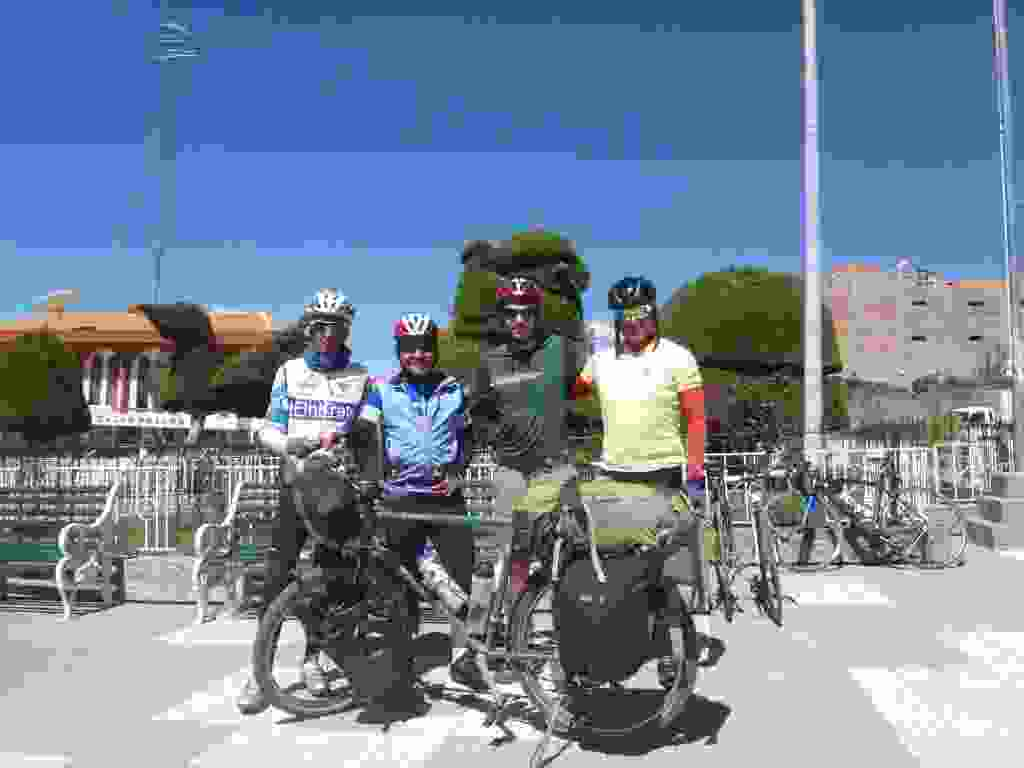
\includegraphics[width=\mywidth]{../wp-content/uploads/2015/05/P5103968-1024x768.jpg} \end{center}

 

 Je reste 2 jours chez Renson qui vit dans un petit appartement. C'est un passionné de vélo et il prépare un voyage en vélo en Europe. 

 

\begin{center} 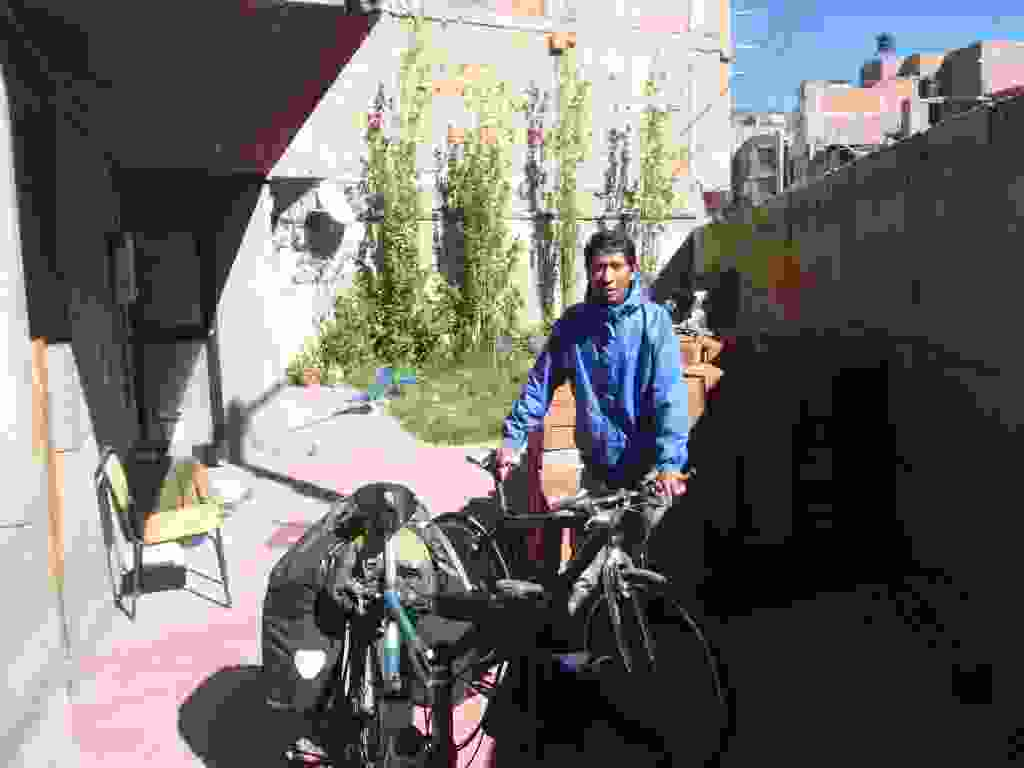
\includegraphics[width=\mywidth]{../wp-content/uploads/2015/05/P5123999-1024x768.jpg} \end{center}

 

 Puno est une ville tranquille avec quelques rues piétonnes. 

 

\begin{center} 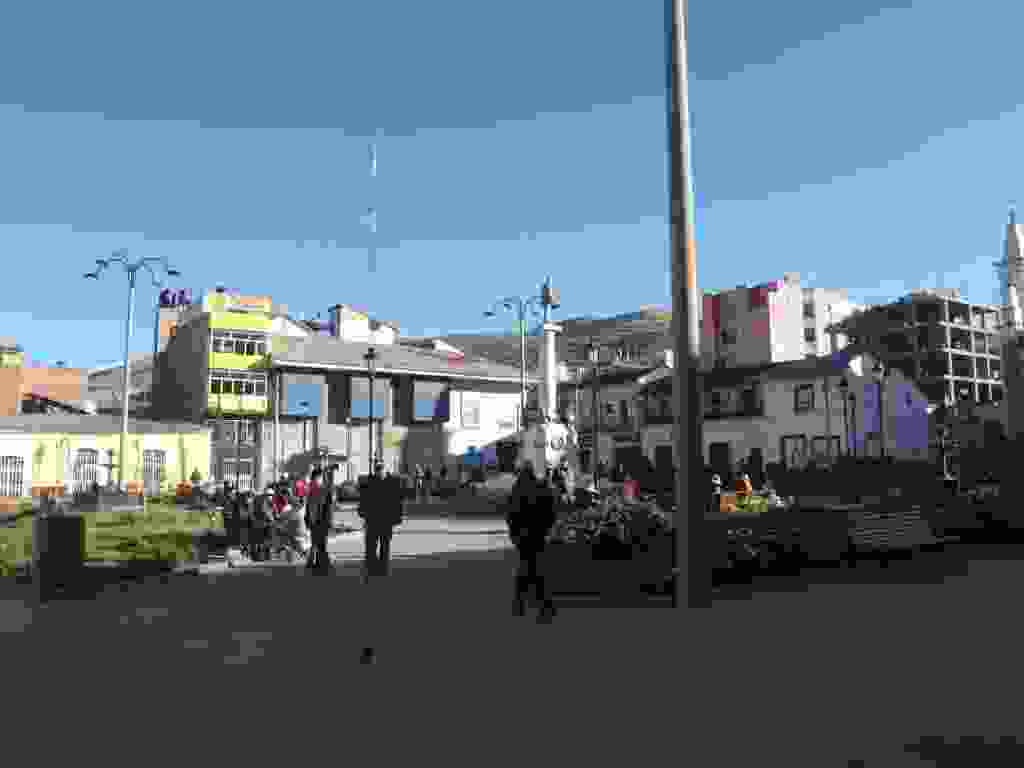
\includegraphics[width=\mywidth]{../wp-content/uploads/2015/05/P5103974-1024x768.jpg} \end{center}

 

 

\begin{center} 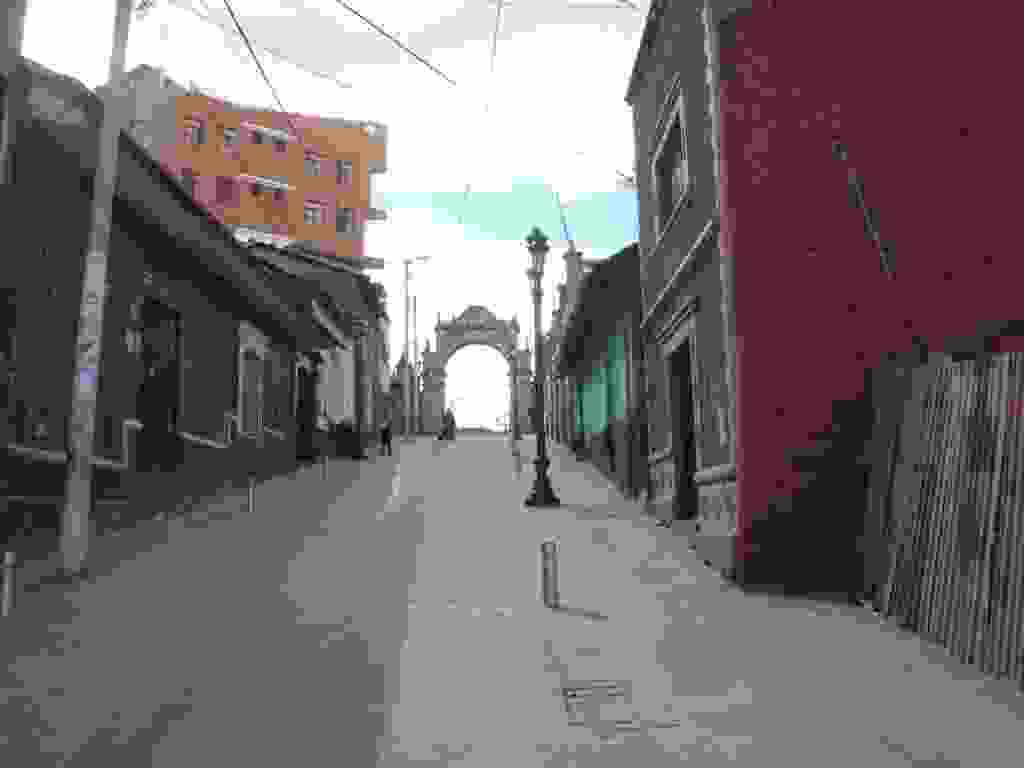
\includegraphics[width=\mywidth]{../wp-content/uploads/2015/05/P5113995-1024x768.jpg} \end{center}

 

 

\begin{center} 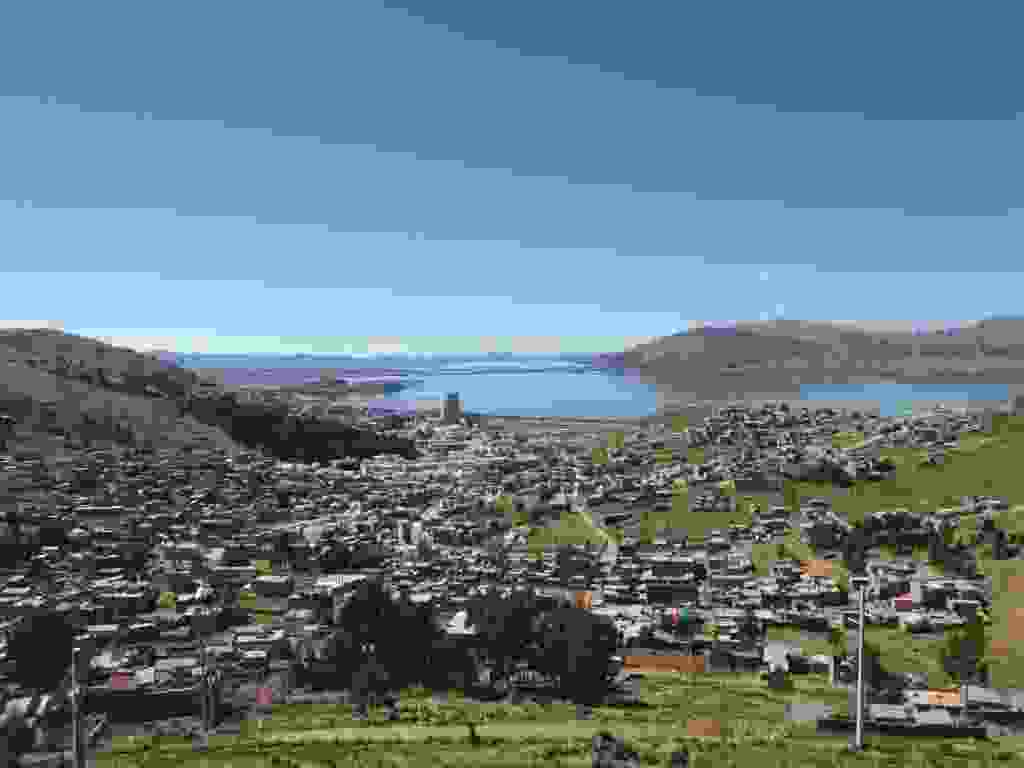
\includegraphics[width=\mywidth]{../wp-content/uploads/2015/05/P5124000-1024x768.jpg} \end{center}

 

 J'ai visité les îles flottantes d'Uros : tout est fabriqué à partir de Totora, un roseau que l'on trouve sur le lac, le sol des îles, les maisons, les bateaux… 

 

\begin{center} 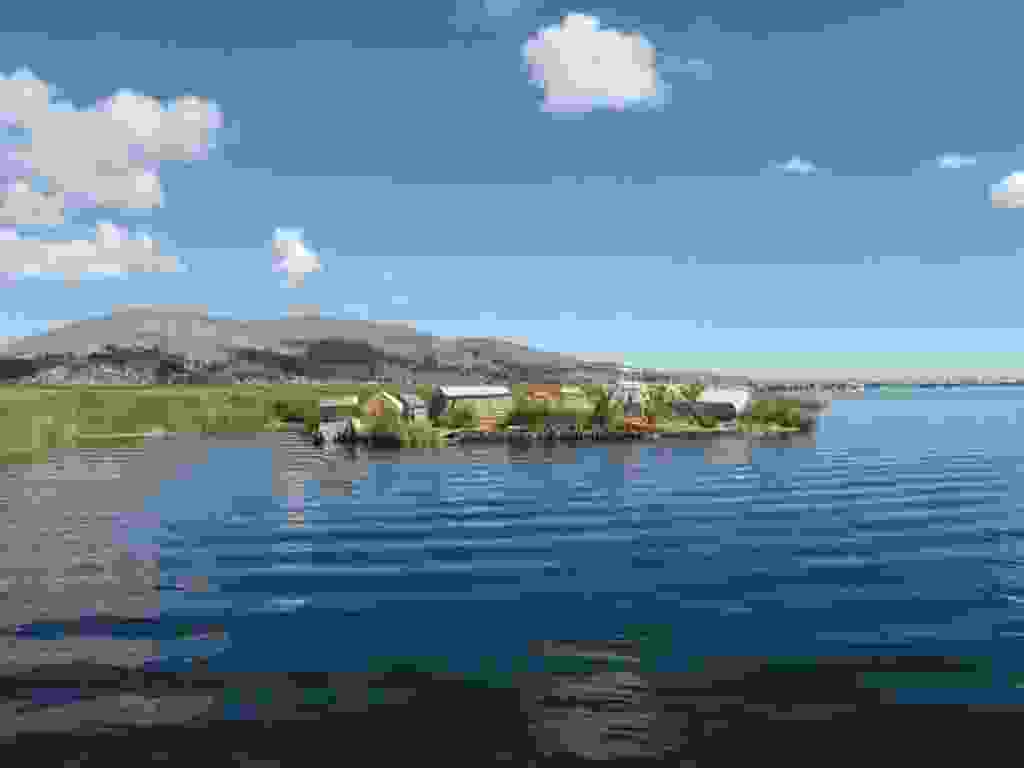
\includegraphics[width=\mywidth]{../wp-content/uploads/2015/05/P5113983-1024x768.jpg} \end{center}

 

 

\begin{center} 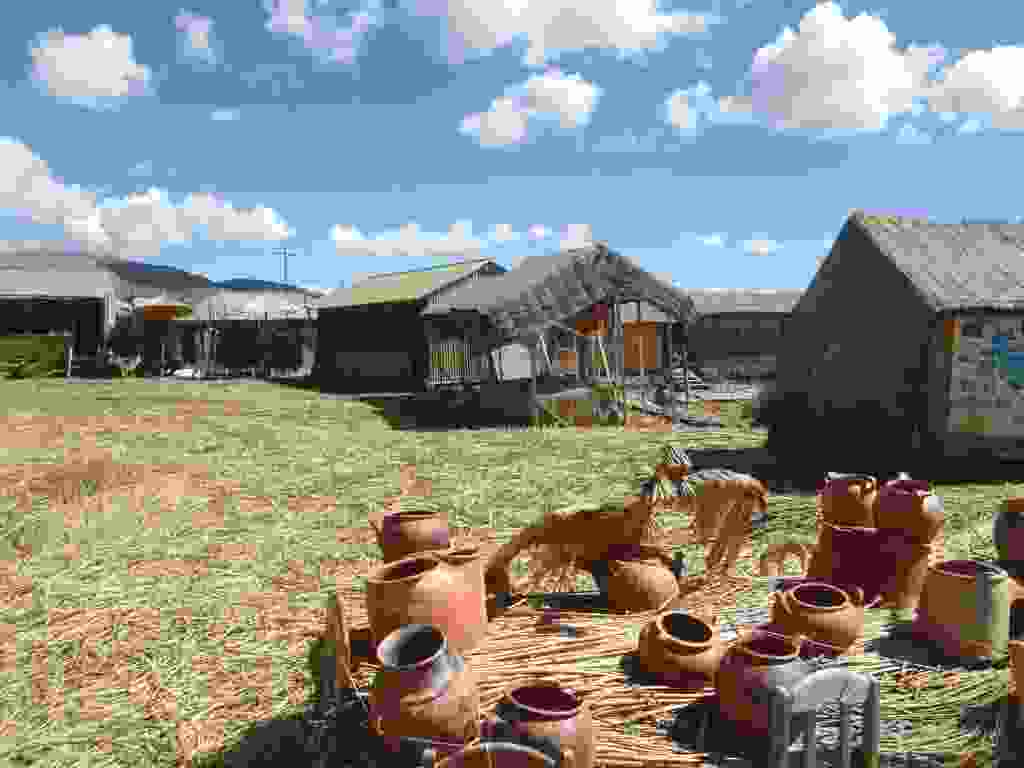
\includegraphics[width=\mywidth]{../wp-content/uploads/2015/05/P5113992-1024x768.jpg} \end{center}

 

 

\begin{center} 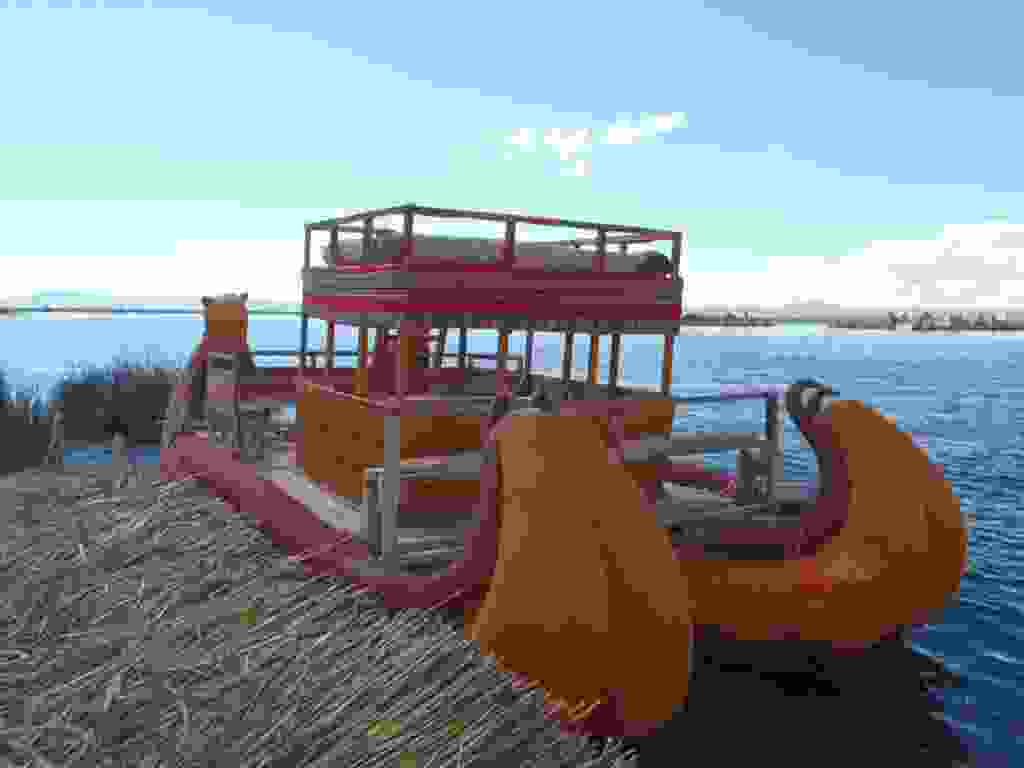
\includegraphics[width=\mywidth]{../wp-content/uploads/2015/05/P5113991-1024x768.jpg} \end{center}




 
 
